\documentclass[a4paper]{report}

\usepackage{amssymb,amsmath,amsfonts}
\usepackage{ntheorem}
\usepackage[usenames]{color}
\usepackage{fancybox}
\usepackage[utf8]{inputenc}
\usepackage[english,russian]{babel}
\usepackage{psfrag}
\usepackage[dvips]{graphicx}
\usepackage[unicode=true,colorlinks=true,pdfstartview=FitH,pdfpagemode=UseOutlines,linkcolor=black,citecolor=black,urlcolor=black,pdftitle={dis},pdfauthor={steve},pdfkeywords={},pdfproducer={LaTeX},pdfcreator={LaTeX}
]{hyperref}
%breaklinks=true]{hyperref}
\usepackage[T2A]{fontenc}
% \usepackage{pscyr}
\usepackage{geometry}
\usepackage{framed}
\usepackage{setspace}
\usepackage{a4}
\usepackage{algorithmic} % noend
\usepackage[boxed]{algorithm} % boxed, ruled, plain (also)
\usepackage[14pt]{extsizes}
\usepackage{iccdisser}
\usepackage{indentfirst}
\usepackage[sorting=none]{biblatex}
\usepackage{color}
\usepackage[usenames,dvipsnames,svgnames,table]{xcolor}
\bibliography{intelle}


\setcounter{tocdepth}{3}  % Точность представления содержания

\setlength{\textwidth}{16.5cm}
\setlength{\textheight}{24cm}

\setlength{\topmargin}{20mm}
\setlength{\headheight}{0mm}
\setlength{\headsep}{0mm}

\setlength{\evensidemargin}{25mm}
\setlength{\oddsidemargin}{25mm}

\setlength{\footskip}{45pt} % Расстояние от нижней грани текста до нижней грани номера страницы
\setlength{\parindent}{10mm} % Абзацный отступ

%\doublespacing
\onehalfspacing

%---------------------------------------------------------------
\begin{document}
%\setlanguage{russian}
\renewcommand\contentsname{Содержание}
\floatname{algorithm}{Процедура}
\renewcommand{\listalgorithmname}{Список процедур}
%\tolerance=5000
%
%
\def\algsty{\nsize\baselineskip=2pt}
\newcommand{\annq}[1]{\textbf{??? - #1}}
\newcommand{\kw}[1]{\texttt{#1}}
\newcommand{\excode}[1]{\texttt{#1}}


\definecolor{code_bk}{rgb}{0.95,0.95,0.95}
\definecolor{note_bk}{rgb}{1,1,0.82}

\newenvironment{code}
{
\fboxrule=1.0pt
\fboxsep=5pt
\renewcommand{\FrameCommand}{\fcolorbox{black}{code_bk}}
\begin{framed}\footnotesize
}
{
\end{framed}
}
\newenvironment{note}
{
\fboxrule=1.0pt
\fboxsep=5pt
\renewcommand{\FrameCommand}{\fcolorbox{black}{note_bk}}
\begin{framed}\sl\footnotesize
}
{
\end{framed}
}

\theorembodyfont{\rmfamily}
\newtheorem{definition}{Определение}
\newtheorem{example}{Пример}
\newtheorem{remark}{Замечание}
\newtheorem{theorem}{Теорема}
\newtheorem{proposition}{Предложение}
\newtheorem{lemma}{Лемма}
\newtheorem{corollary}{Следствие}
%\newtheorem*{proofs}{Доказательство.}

%-------
\newcommand{\fictAquantor}{\ensuremath{\forall\colon\boldsymbol{True}}}
\newcommand{\fictEquantor}{\ensuremath{\exists\colon\boldsymbol{True}}}
\newcommand{\bomega}{\boldsymbol{\omega}}
\newcommand{\bphi}{\boldsymbol{\phi}}
\newcommand{\eqdef}{\stackrel{\mathrm{df}}{=}}
\newcommand{\bigand}[2]{\raisebox{-4pt}{\ensuremath{\overset{#1}{\underset{#2}{\text{\huge\&\normalfont}}}}}}

\definecolor{rclr}{rgb}{0.5,0.1,0.1}
\definecolor{eclr}{rgb}{0,0.5,0.5}
\newcommand{\rem}[2]{\textcolor{rclr}{\framebox{#1}}%
  \ovalbox{\small{}\it{}\color{rclr} #2}%
}
\newcommand{\que}[1]{\rem{#1}{???}}
\newcommand{\app}[1]{\textcolor{eclr}{#1}}

% \sffamily
%\maketitle
%\begin{center}
%\copyright Иркутск 2010
%\end{center}

\begin{titlepage}
%\begin{center}
%    УЧРЕЖДЕНИЕ РОССИЙСКОЙ АКАДЕМИИ НАУК \\
%ИНСТИТУТ ДИНАМИКИ СИСТЕМ И ТЕОРИИ УПРАВЛЕНИЯ \\
%СИБИРСКОГО ОТДЕЛЕНИЯ РАН
%\end{center}
%\vspace{1cm}
\hfill{\vbox{\hbox{На правах рукописи}\hbox{\hfill УДК: 004.4'24:004.896}}}
\vspace{1cm}
\begin{center}
    Ларионов Александр Александрович \\
    \vspace{0.5cm}
\bf ПРОГРАММНАЯ СИСТЕМА АВТОМАТИЧЕСКОГО ДОКАЗАТЕЛЬСТВА ТЕОРЕМ В ИСЧИСЛЕНИИ ПОЗИТИВНО-ОБРАЗОВАННЫХ ФОРМУЛ
\end{center}
\vfill
\hfil\hbox{\hbox{05.13.11 --- }
    \hbox{\vtop{
        \hbox{Математическое и программное обеспечение вычислительных}
        \hbox{машин, комплексов и компьютерных сетей}
    }}%
}\hfil
\vspace{1cm}
\begin{center}
    Автореферат \\
    диссертации на соискание ученой степени \\
    кандидата технических наук
\end{center}
\vfill
%\hfill\hbox{\vbox{
%    \hbox{Научный руководитель}
%    \hbox{к.т.н.~Е.А.~Черкашин}
%}}%
\vfill
\begin{center}
{Иркутск --- 2012}
\end{center}
\end{titlepage}

%
% название ИС
\def\namepc{\hbox{$\rm\mu{}$PrISM}}

\newpage
%=======================================================================================

Работа выполнена в Федеральном государственном бюджетном образовательном учреждении высшего профессионального образования <<Иркутский государственный университет>>

Научный руководитель: кандидат технических наук, доцент Черкашин Евгений Александрович


\newpage
%=======================================================================================

\section*{ОБЩАЯ ХАРАКТЕРИСТИКА РАБОТЫ}

\textbf{Актуальность темы.}
Актуальность..

\textbf{Цель работы} состоит..

\textbf{Основные задачи диссертационной работы:}

\textbf{Методы исселдования.}

\textbf{Научная новизна.}

\textbf{Практическая значимость.}

\textbf{Личный вклад автора.}

%-----------------------------------
\textbf{Апробация работы.}
Основные результаты работы представлены на Международной конференции <<Мальцевские чтения>>, г.Новосибирск, 24-28 августа 2009 г.;
Семинаре ИДСТУ СО РАН <<Ляпуновские чтения>>, ИДСТУ СО РАН, г. Иркутск, 21-23 декабря 2009 г.;
Всероссийской конференции молодых ученых <<Математическое моделирование и информационные технологии>>, г. Иркутск, 15-21 марта 2010 г.;
Международной конференции <<Облачные вычисления. Образование. Исследования. Разработки>>, г.Москва 15-16 апреля 2010 г.;
Международном симпозиуме по компьютерным наукам в России. Семинар <<Семантика, спецификация и верификация программ: теория и приложения>>, г.Казань, 14-15 июня 2010 г.;
4-ой Всероссийской конференции <<Винеровские чтения>>, г.Иркутск, 9-14 марта 2011г.
34-ом международном симпозиуме <<MIPRO>>, г.Опатия, Хорватия, 23-27 мая 2011г.
4-ой Всероссийской мультиконференции по проблемам управления, с. Дивноморское, 3-8 октября 2011г.
13-ой национальной конференции по искусственному интеллекту с международным участием (КИИ-2012), г. Белгород, 16-20 октября 2012 г


%----------------------------------
\textbf{Публикации.} Результаты диссертации отражены в 15 научных работах, в том числе 4 статьи в журналах, рекомендованных ВАК для опубликования научных результатов диссертации на соискание ученой степени доктора или кандидата наук.

%---------------------------------
\textbf{Структура и объём работы.} Диссертация состоят из введения, трёх глав, заключения, библиографии из Н наименований и 4 приложений. Общий объём работы --- 150 страниц, из которых 95 страниц основного текста, включающего 15 рисунков и 2 таблицы.


%=======================================================================================
\section*{СОДЕРЖАНИЕ РАБОТЫ}

\textbf{Во введении} даётся...


%------------------------------------------------------
\textbf{Во второй главе} выделены основные проблемы, требующие тщательного разрешения, а именно: эффективные структуры данных хранения ПО--формул и сопутствующей информации; экономия памяти; неограниченные переменные. 

Для решения перечисленных проблем предложен ряд подходов и стратегий. Дерево состояний вывода


%------------------------------------------------------
\textbf{В третьей главе}...


%------------------------------------------------------
\textbf{В четвёртой главе}...


%------------------------------------------------------
\textbf{А заключении} сформулированы основные результаты, полученные в работе.

%=======================================================================================
\section*{Результаты и выводы}


%=======================================================================================
\section*{Основные положения диссертации опубликованы в следующих работах.}

Работы опубликованные в изданиях, рекомендованных ВАК РФ:

\begin{enumerate}
\item Давыдов А.В., Ларионов А.А., Черкашин Е.А. Об исчислении
позитивно-образованных формул для автоматического доказательства
теорем. // Моделирование и анализ информационных систем. 2010.T. 17, N
4, С. 60--69.
\item Ларионов А.А., Черкашин Е.А., Терехин И.Н. Системные предикаты для
управления логическим выводом в системе автоматического доказательства
теорем для исчисления позитивно-образованых формул. //Вестник
Бурятского государственного университета, 2011, выпуск 9. Серия
Математика. Информатика. с. 94-98.
\item Ларионов А.А., Черкашин Е.А. Параллельные схемы алгоритмов
автоматического доказательства теорем в исчислении
позитивно-образованных формул. // Дистанционное и виртуальное
обучение. Февраль 2012. No. 2, С. 93-100.
\item Davydov A.V., Larionov A.A., Cherkashin E.A. On the calculus of
positively constructed formulas for automated theorem proving. //
Automatic Control and Computer Sciences (AC\&CS). N 1. 2011.
\end{enumerate} 

%---------------------
Работы, опубликованные в других научных изданиях:

\begin{enumerate}
\item A.A. Larionov, E.A. Cherkashin, A.V. Davydov Theorem Proving
Software, Based on Method of Positively-Constructed Formulae. // MIPRO
2011. 34-th international convention on information and communication
technology, electronics and microelectronics. Vol. III. May 23-27,
2011. Croatia, Opatija. //MIPRO: Croatia. - 2011., p.p. 365-368.
\item А.В. Давыдов, А.А. Ларионов. Об исчислении позитивно-образованных
формул для автоматического доказательства теорем. / Тр. 5-го
международного симпозиума по компьютерным наукам в России. Семинар
<<Семантика, спецификация и верификация программ: теория и приложения>>.
14-15 июня 2010, Казань, с. 109-116.
\item Ларионов А.А., Черкашин Е.А., Давыдов А.В. Программная система для
автоматического доказательства теорем в исчислении
позитивно-образованных формул. / Винеровские чтения / Труды IV
Всероссийской конференции. Часть II. - Иркутск: ИрГТУ, 2011. - с.
190-197.
\item А.А. Ларионов, И.Н. Терехин, Е. А. Черкашин, А. В. Давыдов.
Программная система КВАНТ/4 для автоматического доказательства теорем.
// Труды ИМЭИ ИГУ. Математика и информатика : сб.научных трудов / под
ред.: Ю. Д. Корольков [и др.]. - Иркутск : Изд-во ИГУ, 2011. - Выпуск
1 с. 77-85.
\item А.А. Ларионов. Реализация высокопроизводительной системы
автоматического доказательства теорем для метода
позитивно-образованных формул / Тр. Международной конференции
<<Облачные вычисления. Образование. Исследования. Разработки.>>, Москва
15-16 апреля 2010,  с. 63.
\item Ларионов А.А. Методика повышения эффективности обработки
позитивно-образованных формул. / Материалы XI Всероссийской
конференция молодых ученых по математическому моделированию и
информационным технологиям. - Иркутск-Байкал, 15-21 марта 2010,  ИДСТУ
СО РАН.  2010, с. 44.
\item Ларионов А.А. Параллельные стратегии для поиска логического вывода
в исчислении позитивно-образованных формул. / Материалы конференции
<<Ляпуновсякие чтения>>, ИДСТУ СО РАН,  21-23 декабря 2009.
\item Ларионов А.А. Параллельная система автоматического доказательства
теорем в исчислении позитивно-образованных формул. / Вестник
Иркутского Университета, 2009, Иркутск, с. 137-138.
6. А.В. Давыдов, А.А. Ларионов. О стратегиях поиска логического вывода
в исчислении позитивно-образованных формул с функциональными
символами. / Тр. Международной конференции <<Мальцевские чтения>>,
посвященной 100-летию со дня рождения А.И. Мальцева. 24-28 августа
2009, Новосибирск, с. 224.
\item Ларионов А.А., Черкашин Е.А., Давыдов А.В., Хасанов Т.М., Терехин
И.Н. О результатах исследования метода автоматического доказательства
позитивно-образованных формул. / 4-ая Всероссийская мультиконференция
по проблемам управления, <<Искусственный интеллект и управление>>
(ИИУ-2011), 03 - 08 октября 2011, с. Дивноморское, Геленджикский
район, Краснодарский край, Россия.
\end{enumerate}


\newpage
%=======================================================================================
Ларионов Александр Александрович

ПРОГРАММНАЯ СИСТЕМА АВТОМАТИЧЕСКОГО ДОКАЗАТЕЛЬСТВА ТЕОРЕМ В ИСЧИСЛЕНИИ ПОЗИТИВНО-ОБРАЗОВАННЫХ ФОРМУЛ

Автореферат

...

% Введение.
%\chapter{Введение}


%--------------------------------------------
%----------------------об автоматизации рассуждений----------------
%-----------------------------------------------
\section{Об автоматизации рассуждений}
%исторический взгляд
\subsection{Исторический взгляд}
Пионерские идеи об автоматизации (механизации) рассуждений скорее всего высказали Раймунд Луллий (1235-1315) и позднее Готфрид Лейбниц (1646-1716). Луллий описывал некую механическую машину для выведения новых истин, а Лейбниц предложил создать формальный универсальный язык <<lingua characteristica>>, в котором можно было бы формулировать любые утверждения и создать для него исчисление <<calculus ratiocinator>>. Так исчисление могло быть механизированно решать вопрос об истинности утверждений, и это бы стало <<освобождением человеческого разума от его собственных представлений о вещах>>. В качестве примера Лейбниц рассматривал ситуацию, когда два участника спора, для проверки кто из них прав, переводят свои аргументы на <<lingua characteristica>> и потом говорят: <<Calculemus!>> --- подсчитаем. Хотя эти идеи так и остались идеями не найдя никакого материального воплощения, фактически Лейбницом были сформулированы две основных составляющих для автоматизации рассуждений: специальный язык для записи утверждений, который ныне называют <<формальным>> и правила оперирования выражениями этого языка (правила вывода), в совокупности составляющими формальную систему; наличие механизма способного работать с данным языком, в качестве которого сейчас выступает компьютер.
%Появление последних датировано серединой XX-ого века, но к этому времени уже были сформулированы многие принципы формальных систем.

Первая составляющая развивалась в контексте математической логики и оснований математики. Тут стоит указать на роль работ следующих исследователей: Август де Морган, Джордж Буль, Чарльз Пирс, как основоположники логики высказывания и исследователи в области алгебры; Готтлоб Фреге \cite{Frege}, \cite{Sourcebook}, впервые описавший язык и исчисление предикатов (в несколько неестественной для современного человека форме); Джузеппе Пеано, Бертран Рассел, Давид Гильберт, развили результаты Фреге, и поставили важные задачи \cite{GilbertAkkerman}; Курт Гёдель, Алан Тьюринг, Алонзо Черч, получили результаты, касающиеся пределов возможностей формальных систем, в частности полнота \cite{Godel1929} и неразрешимость теорий первого порядка, неполнота систем, выражающих арифметику; Альберт Туральф Сколем, показал что для данного множества истинных высказываний можно механически найти их доказательство; Жак Эрбран доказал, что для истинного математического предложения можно доказать что оно истинно и предложил метод доказательства. В совокупности с результатом Тьюринга и Черча это говорит о полуразрешимости теорий первого порядка.
Идеи Эрбрана и по сей день лежат в основе многих методов.

Вторая составляющая развивалась в контексте вычислительных машин, основным толчком к созданию которых было в большей степени обусловлено выживанием в условиях второй мировой войны, можно отметить работы Джона фон Неймана, Норберта Винера, Алана Тьюринга, Конрада Цузе.

Развитие аппарата математической логики и вычислительных машин естественно привело к созданию первых работающих на практике систем автоматического доказательства теорем: Программа М. Дэвиса в 1954 г. работающая на компьютере <<Johniac>>, доказала что сумма двух четных чисел есть четное число (первое доказательство математического утверждения, произведенное на компьютере) \cite{LogicComp}; <<Логик-теоретик>>, разработанный А. Невелом, Г. Саймоном, Дж. К. Шоу \cite{Newell1}, \cite{Newell2} в 1956 году для доказательства некоторых задач из Principia Mathematica \cite{PrinMat}, причем данная система была направлена на моделирование человеческих рассуждений; В 1958 г. Ван Хао создаёт систему, доказавшую 350 задач из Principia Mathematica \cite{WangHao}.

Началом сильного развития области АДТ явился метод резолюций \cite{Robinson_1965} предложенный Дж.~Робинсоном в 1965 году (работы велись совместно с Д.~Карсоном и Л.~Уосом). Причиной его успеха явилась достаточно хорошая пригодность формализма для реализации на компьютере, в частности однородность представления данных и единственность правила вывода. Стоит отметить что данный метод и по сей день занимает доминирующее положение среди теоретического базиса для систем АДТ.

Отметим что уже в то время указывалось на важность применения эвристик \cite{LogicComp}. И уже тогда зародилась некоторая конкуренция между чисто машинными подходами и эвристическими. В 1960-ые Л.М.~Нортон разработал эвристический прувер для теории групп \cite{LogicComp}.

В 1994 году системой EQP была доказана открытая математическая проблема, что сильно повысило планку возможностей пруверов \cite{McCuneRob}.

О современных системах сказано ниже.

Взятые за базис данной работы первопорядковый язык и исчисление позитивно-образованных формул (ПО--формул) разработаны академиком Васильевым~С.Н., к.ф-м.н. Жерловым~А.К. и академиком Матросовым~В.М. на основе языка типово-кванторных формул, изналчально использовавшегося для формализации свойств динамических систем и синтеза теорем в методе векторных функций Ляпунова.

%Более подробную историческую справку по рассматриваемому вопросу можно найти в работах \cite{LogicComp}, \cite{SourceBook}.

%Добавить про современное состояние дел. %Верификация программного и аппаратного обеспечения, логические и constraint-языки программирования... Приложения АДТ, в т.ч. для логико--динамических систем (Васильев). Или это все дальше есть?

%Формализм по-формул возник как развитие методов... и был предложен в 80-ые годы[], как уже говорилось характерной его чертой является с одной стороны машинная ориентированность, с другой стороны ориентированность на человека. Заметим, что имеется ввиду не просто ориентировнность на какую-то область знаний (типа теории групп, или геометрии) а в принципе на возможность человека вкладывать свои знания в систему. [криво как-то звучит, но суть ясна]. В [КК] дано введение в формализм по-формул а также описаны варианты использования его в задачах интеллектного управления динамическими системами.


\subsection{Область применения систем АДТ}
Первые системы АДТ предназначались скорее для подтверждения возможности автоматизации рассуждений а также для удовлетворения научного интереса авторов. Чуть позднее с появлением логического программирования, интерес перешел в сферу некоторых прикладных проблем искусственного интеллекта ИИ (однако это уже не совсем АДТ).

На сегодняшней день использование АДТ (с обоснованием его эффективности) замечено в следующих областях: верификация программ \cite{ATP_Ver2,keyproj}, синтез программ \cite{Butakov1}, верификация оборудования \cite{ACL2}, обработки естественных языков \cite{ATP_NLP}, решения задач оригами\cite{Origami}, в исследовании protocol languages \cite{tptp}, исследование безопасности информационных потоков \cite{ATP_Flow}, view deletion в базах данных \cite{ATP_DB}, семантическом вебе \cite{tptp}, составлении расписаний \cite{tptp}, задачах управления \cite{ICDS2000}, компьютерном зрении \cite{ATP_Vision} и др.

Наибольшую популярность в настоящее время имеют следующие направления: верификация программных и аппаратных систем; синтез программного обеспечения; решение некоторых проблем математики (библиотека TPTP \cite{tptp}); логическое программирование; дедуктивные базы данных \cite{ontobox}.

%---------------проблемы----
\subsection{Современные системы АДТ и проблемы}

Мы классифицируем системы автоматизации логического вывода следующим образом:
\begin{enumerate}
\item Классические. Предназначены для автоматического доказательств теорем, выраженных языками первого порядка. Отличительной чертой является множество реализованных методик общего характера для повышения эффективности доказательства. Как правило не предназначены для какой-либо специальной предметной области, и могут рассматриваться как универсальные. Наиболее известные из систем: Otter, Vampire (надо добавить, что вампир может компилировать задачу, но он не использует никакой содержательной информации о задаче, просто структуры данных <<статические>> и проиндексированные), EP, SPASS, и др.  В частности  с помощью EQP была доказана открытая математическая проблема \cite{McCuneRob}, а Vampire уже много лет является победителем турнира среди систем АДТ \cite{CASC}. Кроме того, общей чертой данных систем, является использование лишь синтаксической информации о решаемой задаче.

\item Системы, предназначенные для заранее определенного класса задач и неклассических логик. Например для различных алгебраических систем \cite{tptp}, геометрических задач \cite{ATP_geometry, tptp} и др. Характерны тем что либо в принципе предназначены только для указанного класса, либо показывают хорошую производительность на задачах такого класса, но при этом могут быть использованы и для решения других задач. Кроме того, к этому классу могут быть причислены системы АДТ для логик высшего порядка \cite{HOLprover} или скажем для модальных логик \cite{ModalProver}.

\item Настраиваемые (полиморфные) системы. От части к таким системам можно отнести и системы из предыдущих классов, однако под настраиванием мы понимаем в большей степени настройку в соответствии с содержательной информацией о задаче. Как правило, такие системы представляют собой комбинацию существующих систем, например Isabelle \cite{Isabelle} или система предложенная в \cite{ProblemOrientedATP1}. Coq \cite{LaCoq} предлагает использование так называемых <<тактик>>, соединение нескольких типовых шагов вывода в один шаг. Интерактивные системы, хотя и не могут в полной мере быть автоматическими, всё же они интересны тем что используют философию тесного взаимодействия человека и компьютера.
\end{enumerate}
Конечно, некоторые системы могут быть причислены сразу к нескольким классам.


%---------
%Небольшой список с которым мы возможно будет сравниваться: Vampire, Otter, E, SPASS, EQP, Prover9, Isabelle, SNARK, Joke, KeY, ACL2, Coq, NuPRL.
%--------

Из существующих систем АДТ для исчисления ПО--формул, выделим ряд версий системы КВАНТ \cite{dissChe, Che2, QUANT4}, разработанных раннее Е.А.~Черкашиным и его учениками, система Бутакова предназначенная для решения задач разбора LL-1--граммаик \cite{Butakov1}. Предложенная в данной работе система является качественно новой, поскольку все предыдущие могут быть получены из неё путём спецификации. Система Бутакова конкретно предназначено для синтеза разборщика. Система Черкашина была разработана без учета функциональных символов, неограниченных переменных, работы с предикатом равенства, параллельных схем алгоритмов, стратегий экономии памяти и др. В ИДСТУ СО РАН реализованы еще две версии --- Е.Сомова, ориентированная на управление техническими системами, она, фактически, поддерживала очень узкий подкласс ПО--формул и версия Ш.Б.~Гулямова \cite{Gulamov}.

Данные системы относятся ко второму классу систем, согласно классификачии изложенной выше.
%---------

Авторами самых передовых пруверов неоднократно высказывалось что сложность разработки начинает достигать своего предела. Внедряемые методики крайне сложны в реализации, в совмещении с другими методиками, портят расширяемость систему, и вносят абсолютное запутывание в то что происходит внутри системы во время работы. Так, например, в работе \cite{BTPStickel}, автор М.~Стикель (M. Stickel) приводит главу с названием в переводе на русский язык <<Индексирование --- необходимое зло>>, при этом сам М.~Стикель является автором одной из очень популярной и применяемой в самых передовых пруверах методики индексироваия путями (path indexing) \cite{pathindex}.

В работах \cite{Eprover} указывается на то что их система более интеллектна по сравнению с другими системами. Такая интеллектность обусловлена возможностью более гибкого подключения дополнительных эвристик для решения задач определенного класса.

Отсюда можно сказать что, в целом, действительно в области АДТ есть необходимость в новых методах либо в развитии старых в том направлении, чтобы привлекать возможности человека а так же гибкости системы для варьирования своего поведения в зависимости от решаемой задачи.


%--------АКТУАЛЬНОСТЬ---------------
\section{Актуальность исследований}
Отметим что существуют теоремы, которые имеют сколь угодно большой минимальный вывод, т.е., даже если прувер сумеет перебрать все варианты доказательства до определенной глубины, то он всё равно не докажет теорему лежащую вне этого пространства поиска. Отсюда, исследование любых методов, позволяющих расширить возможное пространство поиска (глубину вывода), является актуальным. С нашей точки зрения исчисление ПО--формул как раз даёт фундаментальное сокращение шагов вывода, в силу крупноблочности правила вывода и иерархической структуры.

С другой стороны, такое отодвижение границ даёт лишь потенциальную возможность для доказательства более широкого класса формул. Полный перебор с возрастанием глубины вывода отнимет очень много вычислительных ресурсов. Поэтому так же актуальным является и возможная интеллектуализация процедуры поиска вывода, т.е., дополнительные эвристики о задаче, позволяющие двигаться в предположительно верном направлении поиска.

%Многие современные системы АДТ разрабатываются уже много лет (есть примеры 30-ти летнего опыта), в них внедрено огромное количество методик. Тем не менее эти методики как правило не носят интеллектный характер, а направлены лишь на эффективную обработку данных (например, индексироваие), сокращение потребляемой памяти и т.д. Либо предложен некоторый ограниченный ряд стратегий общего характера.

%Кроме того в силу интеллектности и свойства интерпретируемости вывода в исчислении ПО--формул, было бы интересно разработать методики преобразования формального вывода к виду, пригодному для понимания человеку.

Исходя из изложенных проблем общего характера и классификации существующих систем АДТ для исчисления ПО--формул, в даннй работе акцентируется внимание на разработке системы относящейся к 1 и 3 классу, т.е. с одной стороны повышение производительности автоматической части системы, и разработка инфраструктуры джля взаимодействия с пользователем и подключением дополниетльных стратегйи решения, направленных на конкретную задачу.


%-------------------------------------------------------------------
%---------------- ПО-формулы--------------------------------------
\section{Теоретический базис разработки}

В основе разрабатываемой системы лежит исчисление ПО--формул \cite{ICDS2000}.

Исчисление ПО--формул $\boldsymbol{JF}$ есть тройка $\left\langle \boldsymbol{LF}, Ax\boldsymbol{JF}, \bomega \right\rangle$, где $\boldsymbol{LF}$ --- язык ПО--формул, $Ax\boldsymbol{JF}$ --- единственная схема аксиом и $\bomega$ --- единственное правило вывода $\boldsymbol{JF}.$

%---------------------ЯЗЫК ПО-ФОРМУЛ--------------------
\subsection{Язык позитивно--образованных формул}

Будем обозначать множество всех конъюнктов как $Con$ и положим что {\em конъюнкт} либо конечное множестве обычных атомов языка предикатов первого порядка либо $\boldsymbol{False}$, где $\boldsymbol{False}$ удовлетворяет условию $A \subset \boldsymbol{False} $ для любого $A \in Con$. Пустой конъюнкт обозначается как $\boldsymbol{True}$. Очевидно что если $A \in Con$ тогда $A \cup \boldsymbol{False} = \boldsymbol{False}$. Атомы любого конъюнкта, исключая $\boldsymbol{True}$ и $\boldsymbol{False}$, могут содержать переменные, константные и функциональные символы.

\begin{definition}\label{def:1}
Пусть $\bar{x}$ есть множество переменных и $A$ есть конъюнкт. Правильно-построенные формулы языка ПОФ определяются следующим образом:

Выражение вида $\exists \bar{x}\colon A$ есть $\exists$--формула; выражение вида $\forall \bar{x}\colon A$ есть $\forall$--формула.

Пусть $G_1,\ldots,G_k$ являются $\exists$--формулами, тогда $\forall$--формула имеет следующий вид: $\forall \bar{x}\colon A\left(G_1,\ldots,G_k\right)$.

Пусть $G_1,\ldots,G_k$ являются $\forall$--формулами, тогда $\exists$--формула имеет следующий вид: $\exists \bar{x}\colon A\left(G_1,\ldots,G_k\right)$.

\end{definition}

Выражение является правильно построенной ПО--формулой если оно построено только по правилам Определения \ref{def:1}.

Переменные из $\bar{x}$ связаны соответствующими кванторами и называются $\forall$-переменные и $\exists$-переменные, соответственно.

$\forall$-переменная которая не встречается в соответствующем конъюнкте называется {\em неограниченной} переменной.

%semantic
Теперь определим семантику ПО--формул как семантику соответствующих формул языка предикатов первого порядка.

\begin{definition}\label{def:semantic}
Пусть $A = \{A_1,\ldots,A_l\}$ есть конъюнкт и $\bar{x} = \{x_1,\ldots,x_n\}$ --- множество переменных. Через $A^{\&}$ обозначим $A_1 \&\ldots\&A_l$, при этом $\boldsymbol{False}^{\&}= False, \boldsymbol{True}^{\&}=True$ (пропозициональные константы). Через $F^{\text{\tiny{FOF}}}$ обозначим образ соответствующей ПО--формулы $F$ в языке FOL.

Если $F= \exists \bar{x}\colon A$ то $F^{\text{\tiny{FOF}}} = \exists x_1 \ldots \exists x_n \left(A^{\&}\right).$

Если $F = \forall \bar{x}\colon A$ то $F^{\text{\tiny{FOF}}} = \forall x_1 \ldots \forall x_n \left(A^{\&}\right).$

Если $F = \exists \bar{x}\colon A\left(G_1,\ldots,G_k\right)$ то $F^{\text{\tiny{FOF}}} = \exists x_1 \ldots \exists x_n  \left(A^{\&} \& \left(G_{1}^{\text{\tiny{FOF}}} \& \ldots \& G_{k}^{\text{\tiny{FOF}}}\right)\right).$

Если $F = \forall \bar{x}\colon A\left(G_1,\ldots,G_k\right)$ то $F^{\text{\tiny{FOF}}} = \forall x_1 \ldots \forall x_n \left(A^{\&}\rightarrow \left(G_{1}^{\text{\tiny{FOF}}} \vee\ldots\vee G_{k}^{\text{\tiny{FOF}}}\right)\right).$

\end{definition}

Любая ПО--формула очевидно имеет структуру дерева. Таким образом, для удобства читаемости мы будем представлять их как древовидные структуры а также пользоваться соответствующей терминологии: узел, корень, ветвь, лист и т.д.

Если ПО--формула $F$ начинается с $\forall\colon\boldsymbol{True}$ узла, и каждый лист $F$ является $\exists$--узлом, то $F$ называется ПО--формулой в {\em канонической форме}.
Очевидно что любая ПО--формула $F$ может быть приведена к каноническому виду с помощью следующих преобразований:
\begin{enumerate}
\item Если $F$ не каноническая $\forall$--формула, тогда $\forall\colon \boldsymbol{True}\left(\exists\colon \boldsymbol{True}\left(F\right)\right)$ есть ПО--формула начинающаяся с $\forall\colon\boldsymbol{True}$.
\item Если $F$ есть $\exists$--формула, тогда $\forall\colon \boldsymbol{True}\left(F\right)$ есть ПО--формула начинающаяся с $\forall\colon\boldsymbol{True}$.
\item Если $F$ имеет лист $\forall \bar{x}\colon A$, тогда новый узел $\exists\colon\boldsymbol{False}$ может быть добавлен как потомок.
\end{enumerate}

%В дальнейшем, если не оговорено обратного, будем рассматривать только ПОФы в каноническом виде.

Некоторые части ПО--формул имеют специальные названия: корневой (0-глубины) узел называется {\em корнем} ПО--формулы; любой узел глубины 1 называется {\em базой} ПО--формулы; максимальное поддерево начинающееся с узла глубины 1 называется {\em базовой подформулой}; любой узел глубины 2 называется {\em вопросом} к базе; максимальное поддерево начинающееся с узла глубины 2 называется {\em подформулой-вопросом}; максимальное поддерево начинающееся с узла глубины 3 называется {\em консеквентом}. В соответствии с определением семантики если узел чётной (нечетной) глубины имеет более чем одного потомка, то будем говорить что этот узел имеет {\em дизъюнктивное ветвление} (соответственно {\em конъюнктивное ветвление}).

\begin{example}
Рассмотрим формулу языка FOL
$$F= \neg\bigl(\forall x\:\exists y P(x,y)\rightarrow \exists z P(z,z)\bigr).$$
Образ $F^{\text{\tiny{PCF}}}$ формулы $F$ в языке ПО--формул есть
$$F^{\text{\tiny{PCF}}} = \forall\colon \boldsymbol{True}-\exists\colon\boldsymbol{True} \left\{
\begin{array}{lcl}
 \forall x\colon\boldsymbol{True} & - & \exists y\colon P(x,y) \\
 \forall z\colon P(z,z) & - & \exists\colon\boldsymbol{False}
\end{array}
\right.$$

\end{example}


%-------------------------ИСЧИСЛЕНИЕ ПО-ФОРМУЛ-------------------
\subsection{Исчисление позитивно-образованных формул}

Схема аксиом исчисления ПО--формул $\boldsymbol{JF}$ имеет следующую форму:
$$ Ax\boldsymbol{JF} = \forall\colon\boldsymbol{True}\left(\exists \bar{x}_1\colon\boldsymbol{False}\left(\widetilde{\Phi}_1\right),\ldots,\exists \bar{x}_n\colon\boldsymbol{False}\left(\widetilde{\Phi}_n\right)\right) $$

В исчислении ПО--формул для того что бы доказать $F$ мы будем пытаться опровергнуть её отрицание, поэтому аксиом\app{а} исчисления ПО--формул ---  тождественно ложное высказывание. Таким образом процесс вывода в исчислении ПО--формул является процессом {\em опровержения}.

\begin{definition}
\label{ircond}
Будем говорить что вопрос $\forall \bar{y}\colon A$ к базе $\exists \bar{x}\colon B$ имеет {\em ответ} $\theta$  тогда и только тогда, когда $\theta$ есть подстановка $\bar{y} \rightarrow H^{\infty}$ и $A\theta \subseteq B$, где $H^{\infty}$ есть Эрбранов универсум основанный на $\exists$--переменных из $\bar{x}$, константных и функциональных символах которые встречаются в соответствующей базе.
\end{definition}

%The unique unary inference rule $\bomega$ is defined as follows.

\begin{definition}
\label{omega}
Если $F$ имеет структуру $\forall\colon\boldsymbol{True}\left(\exists \bar{x}\colon B\left(\Phi\right),\Sigma\right)$, где $\Sigma$ есть список других базовых подформул, и $\Phi$ есть список подформул--вопросов содержащий подформулу--вопрос $\forall \bar{y}\colon A(\exists \bar{z}_i\colon C_i\left(\Psi_i\right))_{i=\overline{1,k}}$, тогда заключение $\bomega F$ есть результат применения унарного правила вывода $\bomega$ к вопросу $\forall \bar{y}\colon A$ с ответом $\theta$, и $\bomega F = \forall\colon\boldsymbol{True}(\exists \bar{x} \cup \bar{z}_i\colon B \cup C_i\theta\left(\Phi \cup \Psi_i\theta\right)_{i=\overline{1,k}},\Sigma).$

\end{definition}

После соответствующего переименования некоторых переменных в каждой подформуле, выражение $\bomega F$ будет удовлетворять всем условиям правильно--построенных ПО--формул.

%
Любая конечная последовательность ПО--формул $F, \bomega F, \bomega^2 F,\ldots,\bomega^n F$, где $\bomega^n F \in Ax\boldsymbol{JF}$ называется {\em опровержением} $F$ в исчислении ПО--формул. Иногда будем использовать слово вывод вместо опровержение.

Вопрос с консеквентом $\exists:\boldsymbol{False}$ называется {\em целевым вопросом}. Если вопрос имеет дизъюнктивное ветвление, то ответ на этот вопрос приводит к расщеплению соответствующей базовой подформулы на несколько новых.

Для ясности рассмотрим пример.

\begin{example}[Опровержение в $\boldsymbol{JF}$]\label{proofexample}


\begin{equation*}\label{ex:f1}
	F_1 = \forall\colon\boldsymbol{True} - \exists\colon S(e)(Q_1,Q_2,Q_3,Q_4);
\end{equation*}
\begin{equation*}
	\begin{array}{l}
	Q_1 = \forall x\colon S(x) - \exists\colon A(a) \\
	Q_2 = \forall x,y\colon C(x),D(y) - \exists\colon\boldsymbol{False} \\
	Q_3 = \forall x,y\colon B(x),C(f(y)) - \exists\colon\boldsymbol{False} \\
	Q_4 =
	\forall x\colon A(x) -
	\left\lbrace
	\begin{array}{l}
		\exists y\colon B(y),C(f(x)) \\
		\exists \colon C(x) - \forall z\colon A(z),C(z) - \exists\colon D(f(z))
	\end{array}\right.
	\end{array}
\end{equation*}
На первом шаге вывода существует только один ответ $\{x \rightarrow e\}$ на вопрос $Q_1$. После применения $\bomega$ с этим ответом, формула приобретает следующий вид:
\begin{equation*}\label{ex:f2}
	F_2 = \forall\colon\boldsymbol{True} - \exists\colon S(e),A(a)(Q_1,Q_2,Q_3,Q_4)
\end{equation*}
На втором шаге вывода существует только один ответ $\{x \rightarrow a\}$ на вопрос $Q_4$. После применения $\bomega$ с этим ответом, формула расщепляется, потому что $Q_4$ имеет дизъюнктивное ветвление. И теперь формулы имеет следующий вид:

\begin{equation*}\label{ex:f3}
F_3 =
\forall:\boldsymbol{True} -
\left\lbrace
\begin{array}{l}
	\exists y_1\colon S(e),A(a),B(y_1),C(f(a)) -
	\left\lbrace
	\begin{array}{l}
		Q_1 \\ \cdots \\ Q_4
	\end{array}\right. \\
	\exists\colon S(e)A(a),C(a) -
	\left\lbrace
	\begin{array}{l}
		Q_1 \\ \cdots \\ Q_4 \\
		\forall z\colon A(z),C(z) - \exists\colon D(f(z))
	\end{array}\right. \\
\end{array}\right.
\end{equation*}

На третьем шаге вывода первая база может быть опровергнута ответом $\{x \rightarrow y_1; y \rightarrow a\}$ на целевой вопрос $Q_3$. Опровергнутая база (подформула) для удобства представления может быть удалена из списка базовых подформул.

На четвертом шаге вывода существует ответ $\{z \rightarrow a\}$ на пятый новый вопрос. И формула приобретает следующий вид:
\begin{equation*}\label{ex:f5}
	F_4 = \forall\colon\boldsymbol{True} - \exists\colon S(e),A(a), C(a),D(f(a))
	\left\lbrace
	\begin{array}{l}
		Q_1 \\ \cdots \\ Q_4 \\
		\forall z\colon A(z),C(z) - \exists\colon D(f(z))
	\end{array}\right.
\end{equation*}

На пятом шаге вывода единственная база может быть опровергнута ответом $\{x \rightarrow a; y \rightarrow f(a)\}$ на целевой вопрос $Q_4$.

Опровержение закончено поскольку все базы опровергнуты.

\end{example}

Корректность и полнота доказаны в \cite{}.

%----------------------------------ОСОБЕННОСТИ ПО-ФОРМУЛ--------------------
\subsection{Особенности ПО--формул}
В литературе выделяются различные положительные стороны исчисления ПО--формул. Выделим те, которые, на наш взгляд, являются наиболее подходящими для задачи построения системы АДТ.

\begin{enumerate}
\item\label{flbs} Любая ПО--формула имеет {\em крупноблочную структуру} и только {\em позитивные кванторы} $\exists$ и $\forall$.
%
\item\label{fsimple} Хотя ПО--формулы содержат как квантор $\exists$ так и квантор $\forall$, структура же ПО--формул {\em простая}, {\em регулярная} и {\em предсказуемая} благодаря регулярному чередованию кванторов $\exists$ и $\forall$ по всем ветвям формулы.
%
\item Нет необходимости в предварительной обработке первоначальной формулы первого порядка с помощью процедуры сколемизации (удаление переменных, \app{связанных кванторами существования}. Процедура сколемизации приводит к увеличению сложности термов а значит ив сей формулы. Кроме того, данная особенность делает исчисление более человеко--ориентированным.
%
\item ``Теоретические" кванторы $\forall x$ и $\exists x$ обычно не используются в формализации человеческих знаний, вместо этого чаще используются типовые кванторы $\forall x(A \rightarrow \sqcup)$ и $\exists x(A \& \sqcup)$ \cite{Bourbaki}, \cite{ICDS2000}.
%
\item\label{frule} Исчисление ПО--формул содержит только одно правило вывода и это свойство (как и в случае МР) делает исчисление поболее машинно--ориентированным. Кроме того правило выводя является крупноблочным, что лучше сказывается на человеко--ориентированности.
%
\item\label{froot} Процедура ЛВ фокусируется в ближайшей окрестности корня ПО--формулы, благодаря особенностям \ref{flbs}, \ref{fsimple}.
%
\item\label{fqa} ЛВ может быть представлен в терминах {\em вопросно-ответной} процедуры, а не в технических терминах формального вывода (в терминах логических связок, атомов и др.). Базовый конъюнкт может быть интерпретирован как {\em база фактов}.
%
\item Имеется естественный {\em ИЛИ--параллелизм}.
%
\item\label{fheu} Благодаря \ref{flbs}, \ref{fsimple}, \ref{froot}, \ref{fqa} процедура ЛВ {\em хорошо совместима с конкретными эвристиками приложения}, а также с эвристиками общего управления выводом. Благодаря \ref{frule} доказательство состоит из крупноблочных шагов, и оно хорошо {\em наблюдаемо} и {\em управляемо}.
%
\item Благодаря \ref{fqa}, \ref{fheu} доказательство может быть интерпретировано человеком.
%
\item Семантика исчисления ПО--формул может быть изменена без какой либо модификации аксиом или правила вывода $\bomega$. Такая модификация реализуется просто путём ограничений на применение правила вывода $\bomega$ и позволяет трансформировать классическую семантику исчисления ПО--формул в немонотонную, интуиционистскую, и т.п. Примеры использования таких семантик представлены в \cite{ICDS2000}.
\end{enumerate}


%-------------------------------------------------------------
%------------------------------------------------------------
\section{Формальная информация о диссертации}

% Объект — это процесс или явление, порождающее проблемную ситуацию и взятое исследователем для изучения. Предмет — это то, что находится в рамках, в границах объекта. Объект — это та часть научного знания, с которой исследователь имеет дело. Предмет исследования — это тот аспект проблемы, исследуя который, мы познаем целостный объект, выделяя его главные, наиболее существенные признаки. Предмет диссертационного исследования чаще всего совпадает с определением его темы или очень близок к нему. Объект и предмет исследования как научные категории соотносятся как общее и частное.

%----------------
\paragraph{Объектом исследования}\hspace{-1em} является разработка эффективных алгоритмов и программного обеспечения для автоматического доказательства теорем в исчислении ПО--формул. В работе производится повышение эффективности АДТ по следующим критериям: сокращение времени решения задач; экономное использование оперативной памяти; минимизация количества шагов логического вывода; расширение класса решаемых задач. %Или это таки предмет уже???

%----------------
\paragraph{Предметом исследования}\hspace{-1em} являются разработка методик повышения производительности логического вывода в исчислении ПО--формул, оригинально разработанные или адаптированные из существующих систем АДТ.

%-----------------??
%\paragraph{Методика исследования.}\hspace{-1em} Использование исчисления ПО--формул как базиса для АДТ; Использование языка D для программирования системы; Анализ других систем АДТ на предмет применения их методов.

%-----------------??
\paragraph{Цель диссертационной работы:}\hspace{-1em} Разработка высокопроизводительной программной системы для автоматического доказательства теорем в исчислении позитивно--образованных формул.

%-----------------??
\paragraph{Основные задачи диссертационной работы.} Для достижения описанной выше цели решаются следующие задачи:
\begin{enumerate}
\item Исследование языка и исчисления ПО--формул, анализ его свойств, влияющих на возможность адаптации существующих алгоритмов и разработки новых алгоритмов;
\item Разработка эффективных структур данных представления ПО--формул в памяти компьютера;
\item Разработка алгоритмов преобразования ПО--формул для организации автоматического логического ввода;
\item Адаптация существующих методик реализации алгоритмов АДТ для исчисления ПО--формул;
%\item Разрешение основных проблем исчисления ПО--формул, негативно влияющих на эффективность автоматического поиска ЛВ;
\item Исследование вопросов автоматизации построения эффективного логического вывода с использованием предиката равенства;
\item Разработка программной системы АДТ, создание инструментальных средств для программирования специальных версий АДТ, ориентированных на определенные классы теоретических и практических задач поиска ЛВ.
%\item Реализация программной инфраструктуры, обеспечивающей человеку возможность управления процессом поиска логического вывода;
\item Апробация разработанных программных средств в решении тестовых и практических задач.
\end{enumerate}

%-------------------------------------------------------------------
%------НАУЧНАЯ НОВИЗНА, ПРАКТИЧЕСКАЯ ЗНАЧИМОСТЬ, АПРОБАЦИЯ----
%------------------------------------------------------
%-----??
\paragraph{Научная новизна выполненных исследований}
Разработаны новые и адаптированы существующие алгоритмы, реализующие метод АДТ для реализации исчислений ПО--формул. Использование данных алгоритмов позволило реализовать полноценную программную систему АДТ для этих исчислений. В результате проведенного исследования получены следующие новые научные результаты:
\begin{enumerate}
\item Изучены свойства исчисления ПО--формул, определяющие характер адаптации существующих алгоритмов;
\item Предложены и реализованы ряд стратегий поиска логического вывода ПО--формул с неограниченными переменными;
\item Предложена и реализована стратегия $k,m$--ограничения;
\item Усовершенствован подход к представлению структур данных ПО--формул в направлении использования разделения оперативной памяти;
\item Адаптированы алгоритмы индексирования термов для системы АДТ ПО--формул;
\item Предложены и реализованы стратегии параллельного логического вывода для системы АДТ ПО--формул;
\item Предложен подход для работы с предикатом равенства, без прямого представления аксиом равенства в виде ПО--формулы.
\end{enumerate}

%--------------------??
\paragraph{Практическая значимость}\hspace{-1em} представляется следующими основными результатами:
\begin{enumerate}
\item Разработана система АДТ и инструментальная среда разработки систем АДТ, направленных на решения специальных классов задач.
\item Выделены классы задач, на которых разработанная система ведёт себя более эффективно чем самые производительные современные системы АДТ, предложены специальные стратегии поиска ЛВ для этих классов;
\item Реализована инфраструктура тестирования разработанных алгоритмов и программного обеспечения АДТ на тестовых задачах TPTP; % Это совсем частная задача.
%\item Расширена область применения систем АДТ (Леса? или ИСИ).
%Надо, чтобы корреляция была с поставленными задачами.
\end{enumerate}

Кроме того, немаловажным результатом является возможность использования системы АДТ базирующейся на раннее не использованном исчислении ПО--формул (новый взгляд на задачи).

Работы и исследования, проведенные в рамках  диссертации, выполнены в ФГБОУ ВПО <<Иркутский государственный университет>> и в Институте динамики систем и теории управления СО РАН.

Исследования поддержаны федеральной целевой программой, базовым финансированием СО РАН и грантами:
\begin{enumerate}
\item Федеральная целевая программа «Научные и научно--педагогические кадры инновационной России» на 2009-2013 годы, госконтракт № П696;
\item Базовые проекты научно--исследовательской работы ИДСТУ СО РАН. Проект IV.31.2.4. ``Методы и технологии разработки программного обеспечения для анализа, обработки, и хранения разноформатных междисциплинарных данных и знаний, основанные на применении декларативных спецификаций форматов представления информации и моделей программных систем'',№ гос. регистрации: 01201001350. Программа IV.31.2. ``Новые ГИС и веб--технологии, включая методы искусственного интеллекта, для поддержки междисциплинарных научных исследований сложных природных, технических и социальных систем с учетом их взаимодействия'', . Проект IV.32.1.2. Информационно-вычислительные системы нового поколения для формаций автономных необитаемых аппаратов, № гос. регистрации: 01201001346;
\item РФФИ 08-07-98005-р\_сибирь\_а <<Программные технологии логико--математического моделирования динамики лесных ресурсов Байкальского региона>>;
\item Программа <<Университетский кластер>>.
%\item MIPRO канает?
\end{enumerate}

Разработанные инструментальные средства внедрены в учебный процесс вузов города Иркутска, в частности, в Институте математики, экономики и информатики Иркутского государственного университета (ИМЭИ ИГУ). Разработана новый вариант курса ``Технологии разработки программного обеспечения'' на кафедре информационных технологий ИМЭИ ИГУ.

\paragraph{Результаты, выносимые на защиту}\hspace{-1em} представляется следующими основными результатами:

% Где внедрены разработанные инструментальные средства.

% ??? внедрение на производстве и в фирмах

% ??? Собственное применение.



%------------------------------------------
\paragraph{Представление работы.} Материалы работы докладывались на
\begin{itemize}
\item Международной конференции <<Мальцевские чтения>>, г.Новосибирск, 24-28 августа 2009 г.;
\item Семинаре ИДСТУ СО РАН <<Ляпуновские чтения>>, ИДСТУ СО РАН, г. Иркутск, 21-23 декабря 2009 г.;
\item Всероссийской конференции молодых ученых <<Математическое моделирование и информационные технологии>>, г. Иркутск, 15-21 марта 2010 г.;
\item Международной конференции <<Облачные вычисления. Образование. Исследования. Разработки>>, г.Москва 15-16 апреля 2010 г.;
\item Международном симпозиуме по компьютерным наукам в России. Семинар <<Семантика, спецификация и верификация программ: теория и приложения>>, г.Казань, 14-15 июня 2010 г.;
\item 4-ой Всероссийской конференции <<Винеровские чтения>>, г.Иркутск, 9-14 марта 2011г.
\item 34-ом международном симпозиуме <<MIPRO>>, г.Опатия, Хорватия, 23-27 мая 2011г.
\item 4-ой Всероссийской мультиконференции по проблемам управления, с. Дивноморское, 3-8 октября 2011г.
\item 13-ой национальной конференции по искусственному интеллекту с международным участием (КИИ-2012), г. Белгород, 16-20 октября 2012 г.
\end{itemize}

%-------------------------------
\paragraph{Публикации по теме диссертации.} По теме диссертации опубликовано 3 работы в журналах из перечня рецензируемых научных журналов и изданий ВАК, в которых публикуются научные результаты диссертации на соискание ученой степени доктора и кандидата наук, и Web of Science:
\begin{enumerate}
\item Давыдов А.В., Ларионов А.А., Черкашин Е.А. Об исчислении
позитивно-образованных формул для автоматического доказательства
теорем. // Моделирование и анализ информационных систем. 2010.T. 17, N
4, С. 60--69.
\item Ларионов А.А., Черкашин Е.А., Терехин И.Н. Системные предикаты для
управления логическим выводом в системе автоматического доказательства
теорем для исчисления позитивно-образованых формул. // Вестник
Бурятского государственного университета, 2011, выпуск 9. Серия
Математика. Информатика. с. 94-98.
\item Ларионов А.А., Черкашин Е.А. Параллельные схемы алгоритмов
автоматического доказательства теорем в исчислении
позитивно-образованных формул. // Дистанционное и виртуальное
обучение. Февраль 2012. No. 2, С. 93-100.
\item Davydov A.V., Larionov A.A., Cherkashin E.A. On the calculus of
positively constructed formulas for automated theorem proving. //
Automatic Control and Computer Sciences (AC\&CS). 2011. Volume 45, Issue 7, pp.~402-407.
\end{enumerate}

%---------------------------------
\paragraph{Личный вклад автора.} Все представленные результаты получены лично автором или в соавторстве с научным руководителем Черкашиным~Е.А. и Давыдовым~А.В. Автором лично разработаны:
\begin{enumerate}
\item Разработка стратегий поиска ЛВ, являющихся основой разработанных алгоритмов;
\item Разработка и адаптация алгоритмов поиска логического вывода в исчислении ПО--формул;
\item Реализация структур данных для представления ПО--формул;
\item Реализация программной системы АДТ;
\item Тестирование системы АДТ на тестовых примерах АДТ.
\end{enumerate}

Совместно с Черкашиным Е.А. проведена разработка структур данных для представления ПО--формул с использованием разделения оперативной памяти. Совместно с Давыдовым А.В. созданы методики поиска ЛВ с использованием неограниченных переменных.

Из печатных работ, опубликованных диссертантом в соавторстве, в текст глав 2,3 и 4 диссертации вошли только те результаты, которые содержат непосредственный определяющий (10/4) творческий вклад автора диссертации на этапах проектирования и разработки программного обеспечения. В перечисленных публикациях все результаты, связанные с вопросами реализации и использования программной системы принадлежат автору.

%-------------------------------------
\paragraph{Соответствие паспорту специальности}
05.13.11 -- Математическое и программное обеспечение вычислительных машин, комплексов и компьютерных сетей. Область исследования 5. Программные системы символьных вычислений; 8. Параллельное программирование.

%-------------------------------
\paragraph{Структура и объем диссертации.} Диссертация состоит из четырех глав, первая из которых --- вводная, заключения, списка литературы и приложения. Основной текст изложен на \pageref{pg:main} страницах машинописного текста, полный объем диссертации \pageref{pg:total} страниц. В работе содержится 12 рисунков. Список литературы содержит 65 наименований.

Глава 2 посвящена представлению методик повышения производительности АДТ, разработанным стратегиям поиска ЛВ, базису программной системы. Выделены некоторые проблемы ПО--исчисления, решение которых требовалось для эффективных реализаций разработанных стратегий. Представлен ряд стратегий, адаптированных из существующих систем АДТ и новые стратегии для исчисления ПО--формул, рассмотрен вопрос решения задач с предикатом равенства.

Глава 3 посвящена аспектам реализации и использования системы. Представлены системные предикаты управления ЛВ, реализация арифметики, трансляторы с различных языков представления первопорядковых формул.

В главе 4 представлены методы и результаты тестирования системы. В частности дано описание библиотеки TPTP и некоторых задач, представленных в этой библиотеке. %Решена задача о лесах с применением внешних эвристик.

В заключении приводится список результатов, полученных в диссертации. % выносимых на защиту.

Приложение содержит описание грамматики входного языка, пример протокола вывода для решения задач, сводную информацию о решенных задач из библиотеки TPTP.

%--------благодарности-------------
\paragraph{Благодарности.} Автор благодарит к.т.н. Черкашина~Е.А. за руководство диссертационной работой и помощь в подготовке рукописи, Давыдова~А.В. за ценные указания в работе.


%%% Local Variables:
%%% mode: latex
%%% TeX-master: "dis"
%%% End:

% Алгоритмы
%\chapter{Алгоритмическое обеспечение и адаптация алгоритмов}

В этой главе рассматривается задача адаптации существующих алгоритмов,
используемых в различных системах АДТ для повышения производительности
процесса поиска логических выводов, \app{а также разработка других
специализированных алгоритмов}. В результате адаптации получены \rem{...}{Что в результате получается..}

%==========================================================
\section{Предпосылки разрабатываемых алгоритмов}

Для того что бы алгоритмы адекватно использовали возможности
ПО--формализма необходимо выявить его основные полезные свойства, а также свойства, не совместимые с адаптируемыми алгоритмами.  Полезные свойства представлены во введении и являются общепризнанными.

%--------------------ПРОБЛЕМЫ------------------------------------
\subsection{Проблемы формализма ПО-формул}
Укажем на некоторые свойства ПО-формализма, сказывающиеся на
\rem{производительности процесса поиска ЛВ и ...}{Как оно сказывается?} в частичном разрешении которых он нуждается.

\begin{enumerate}

\item Поиск ответов на вопросы с открытыми переменными требует выбора
  подставляемого терма для данной переменной из эрбранова универсума,
  который в общем случае, т.е. при наличии функциональных символов, является бесконечным множеством (счетным множеством). Какой именно терм необходимо выбрать --- изначально неизвестно.

Сделаем несколько замечаний. Во-первых, при решении прикладных задач, переменные связанные квантором всеобщности ограничиваются типовым условием, а значит появление открытых переменных в данном случае следует рассматривать как некую аномалию в следствии неверной формализации задачи. Это значит, что решение данной проблемы лежит вне прикладной области, и необходимо для решения общематематических теорем (например из библиотеки TPTP).  Во-вторых, есть соблазн уйти от функциональных символов (как это скромно сделано в \cite{Vas_ICDS}), но наличие функциональных символов есть основа сложных задач. В-третьих, в \cite{Vas_ICDS} предложена идея стратегии решения данной проблемы --- стратегия отсроченного присваивания (СОП), заключающаяся в том что изначально для открытой переменной выбирается неопределенный эрбранов элемент, а позднее он постепенно доопределяется. Подробное описание стратегии и её реализация представлены в главе 3. Данная стратегия конфликтует с другими стратегиями. Однако анализ решаемых задач показывает что в прикладных задачах (как-то их иначе наверное надо назвать) нет нужды использовать СОП ибо нет открытых переменных, а в общих задачах сложнее найти какие-то особенности которые применяются другими стратегиями, а значит конфликт частично разрешается просто разграничением областей применения системы.

\item Язык ПО-формул позиционируется как <<достаточно однородной, но в то же время хорошо структурированный>> и хорошо усваивающий эвристики. Стоит заметить, что однородность ПО-формул хуже чем, например, однородность дизъюнктов, в силу разнородных сущностей структуры формулы: база, вопросы, консеквенты вопросов. Разрешение данного вопроса требует применения специальных методов доступа к данным неоднородным частям.

\item Хотя изначально представление формулы ИП в языке ПО-формул более компактно чем КНФ, дальнейшее проведение правила вывода может привести к бОльшему усложнению структуры формулы (при наличии дизъюнктивного ветвления), чем при применении правила вывода в МР. Таким образом через некоторое количество шагов ввода размер ПО-формулы может оказаться в разы больше чем размер КНФ. Но эта проблема почти полностью устранима чисто техническими способами, а именно описанными далее методами разделения данных, а также ограничивающей стратегией (которую пользователь выбирает сам).

\end{enumerate}


%---------------------------
\subsection{Подходы}
Поскольку в данной работе рассматривается первопорядковый язык ПО-формул, некоторые из структур данных и алгоритмов имеют сходства с уже существующими системам АДТ первого порядка. Это касается структуры термов и подстановок. Кроме того существуют общетехнические методы независящие от конкретного формализма, например параллельные схемы алгоритмов, экономия потребляемой памяти, индексирование данных.

Таким образом в работе предполагается адаптация некоторых существующих алгоритмов, используемых в современных и самых эффективных системах АДТ. Адаптация предполагает, во-первых, учет особенностей ПО-формализма - как положительных так и проблемных, во-вторых, совмещение (синхронизация) алгоритмов, поскольку некоторые из них конфликтуют при прямой реализации.



%===============================================================
%---------------------------------------------------------------
%-----------------------АЛГОРИТМЫ---------------------------
\section{Алгоритмы и структуры данных}

%===================базовые структуры данных========================
\subsection{Общие структуры данных}

\textbf{Типы данных.} Язык представления формул имеет следующие типы данных: ATOM (атомарный символ), FUNCTION (функциональный символ), CONSTANT (константный символ), AVARIABLE (универсальная переменная), EVARIABLE (экзистенциальная переменная), UHE (Неопределённый Эрбрановский Элемент), INTEGER (целочисленный символ), FLOAT (нецелочисленный символ), STRING (строковый символ). Данные типы определяются перечислением:

{\tt enum SymbolType {CONSTANT, EVARIABLE, AVARIABLE, FUNCTION, ATOM, INTEGER, FLOAT, STRING, UHE};}


\textbf{Символ (Symbol).} Символ - буква из алфавита используемого языка. Структура Symbol содержит строковое представление символа, тип данных, арность. Символ идентифицируется по его адресу в памяти.

\textbf{Обобщённый терм (GTerm).} Такое название взято из \cite{NNN}. Смысл заключается в том что для представления как терма так и атома используется одна структура данных, поскольку и первые и вторые имеют древовидную структуру. Для правильной обработки соответствующих обобщенных термов используются вышеописанные типы данных. Терм представляется классической древовидной структурой каждый узел которой содержит символ верхнего уровня и массив ссылок на дочерние узлы. Универсальная переменная (AVARIABLE) и неопределённый эрбрановский элемент (UHE) используют один дочерний узел как ссылку на терм, который подставляется вместо данного. Если ссылка не UML значит переменная связана с некоторым термом. В противном случае переменная свободная для подстановки. Для того что бы корректно обрабатывать переменные, задан метод getValue() который возвращает значение типа GTerm. Если переменная не связана то значение getValue() совпадает со ссылкой на эту переменную, в противном случае возвращается ссылка на терм с которым связана переменная.

\textbf{Чанк.} Маркированный список. Список разделённый на подсписки любой длины (в том числе нулевой). Для каждого элемента списка можно определить к какому подсписку он относится. Далее будет показано что в каждом чанке хранится информация о текущем шаге выводе, а весь список в целом хранит всю информацию о формуле. Т.е. формула это список, а чанк это подформула полученная на определённом шаге вывода. На рисунке представлена структура чанкового списка.

\begin{figure}[h]
	%\vspace{0.5cm}
	\centering
	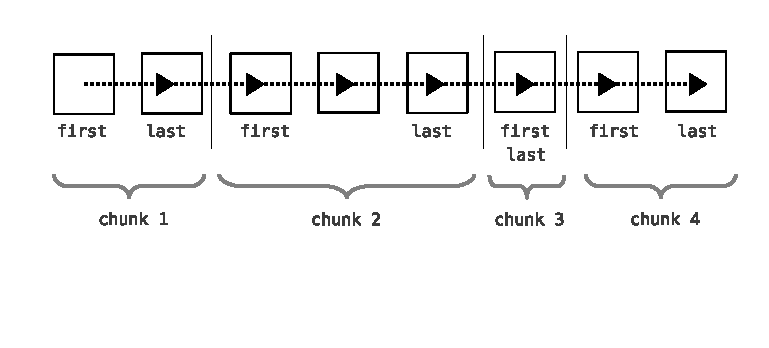
\includegraphics[width=0.6\linewidth]{pics/Chunk.eps}
	\caption{Чанковый список}
	\label{fig:chank1}
\end{figure}

На следующем рисунке показан случай когда один из чанков пуст.

\begin{figure}[h]
	%\vspace{0.5cm}
	\centering
	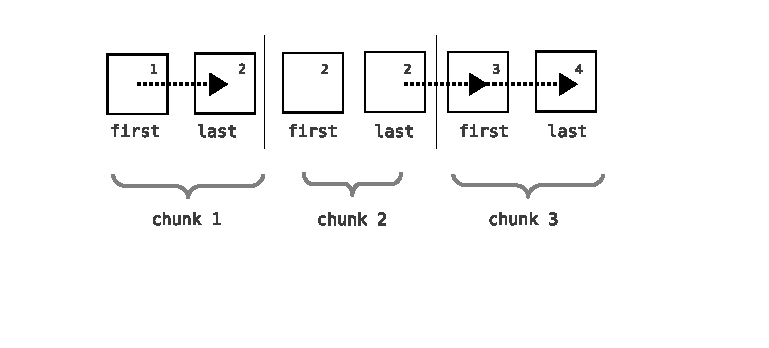
\includegraphics[width=0.6\linewidth]{pics/Chunk2.eps}
	\caption{Чанковый список}
	\label{fig:chank2}
\end{figure}

Стоп.


%=================== ДЕРЕВО СОСТОЯНИЙ ВЫВОДА =======================
\subsection{Дерево состояний вывода}
Одним из основополагающих методов в разработанной системе АДТ является дерево состояний вывода (ДСВ), состоящее из структур данных, характеризующих логический вывод и ряда методов, обрабатывающих данные структуры. Основная цель данного подхода заключается в том что бы строго зафиксировать все события произошедшие на каждом шагу логического вывода, например что бы точно определить какие данные были выведены на каком шагу вывода. Такая фиксация событий позволит:
\begin{enumerate}
 \item Более глубоко анализировать процесс ЛВ, а значит эффективно внедрять эвристики.
 \item Производить откаты в выводе (backtracking).
 \item Реализовать один из подходов разделения данных.
 \item Производить эффективное освобождение памяти.
\end{enumerate}

Для начала, кратко объясним идею ДСВ.
При классическом подходе после каждого ответа на вопрос к первоначальной формуле добавляется консеквент вопроса на который производился ответ (в базу добавляются соответствующие элементы узлов непосредственно следующих за вопросом; к вопросам добавляются новые вопросы, если они есть), а в случае дизъюнктивного ветвления соответствующая база расщепляется, не теряя никаких данных.
Таким образом, формула монотонно увеличивается, при этом сохраняя свою структуру.
ДСВ будем использовать для того что бы иметь полную информацию о текущей формуле, для возможности отката в выводе и подробного наблюдения за ним. Опишем ДСВ формально.

Дерево состояний вывода есть такое дерево, которое обладает следующими свойствами: корень дерева есть одна из базовых подформул первоначальной формулы; все остальные узлы есть добавляемые консеквенты (с примененным к ним подстановками-ответами и разыменованием переменных). Если приводить в пример определение правила вывода, то корень дерева это база E, а узлы это E2theta.
Таким образом если происходит расщепление то в данном узле появляется ветвление.
Отсюда можно говорить что каждая базовая подформула в формуле характеризуется соответствующим путём от листа до корня.

Как видно, каждый узел содержит самодостаточную информацию и для того чтоб производить откаты назад, достаточно удалять соответствующие узлы.
Кроме того такой подход реализует разделение данных (ссылок) на каждый консеквент, поскольку некоторые пути могут иметь общие подпути.
Если какая-то база опровергнута, то можно удалить все узлы от соответствующего листа до ближайшего ветвления, поскольку оставшаяся часть пути всё ещё используется для представления другой базы. Количество узлов равно текущему количеству баз. Если дерево пусто, значит первоначальная база опровергнута.
Та как изначальная формализация задачи в языке ПО-формул может содержать несколько базовых подформул, то для каждой из этих подформул строится своё ДСВ.

Для практических нужд узел ДСВ содержит некоторую системную информацию:
\begin{enumerate}
\item Множество атомов, понимаемых как часть базовых, отсюда каждый базовый конъюнкт характеризуется объединением всех множеств от данного узла до корня.
\item Список ссылок на вопросы к базе.
\item Для каждого вопроса определяется чанк ответов для вопроса в данный момент.
\item Номер последующего шага вывода и соответствующий ответ, если узел имеет потомков.
\item Чанк уже отработанных вопросов.
\end{enumerate}

Узлы содержат ещё различную информацию, которая будет описана ниже в описании стратегий вывода.

За счёт чанков получается разграничивать данные полученные на каждом шаге, с другой стороны на каждом шаге (в каждом узле) доступные все собранные до этого данные.

ДСВ для формулы из примера представлено на рисунке Рис.~\ref{fig:pst}.
Корнем ДСВ является первоначальная ПО-формула $F_1$. Узел ``2" является консеквентом вопроса $Q_1$, а именно $\exists\colon A(a)$, а путь от узла 2 до корня соответствует ПО-формуле $F_2$. Узлы 3 и 4 являются соответствующими консеквентами для вопроса $Q_4$. Путь от узла 3 до корня и путь от узла 4 до корня соответствуют базовым подформулам ПО-формулы $F_3$. Например, формулы определённые путями 5 --- 1 и 3 --- 1 разделяют данные которые представлены узлами 1 --- 2. Когда базовая подформула, которая представлена узлами пути 3 --- 1 опровергнута, то можно удалить путь от узла 3 до ближайшего ветвления (в сторону корня) --- в данном случае удаляется только узел 3, поскольку узлы 2 --- 1 всё ещё используются для представления других базовых подформул.

\begin{figure}[h]
	%\vspace{0.5cm}
	\centering
	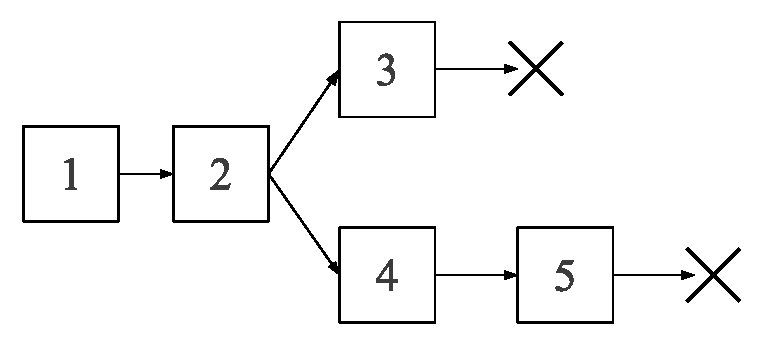
\includegraphics[width=0.4\linewidth]{pics/PST.eps}
	\caption{Дерево состояний вывода для формулы из примера \ref{proofexample}.}
	\label{fig:pst}
\end{figure}

На следующем рисунке представлено ДСВ с точки зрения его связи с чанками.

\begin{figure}[h]
	%\vspace{0.5cm}
	\centering
	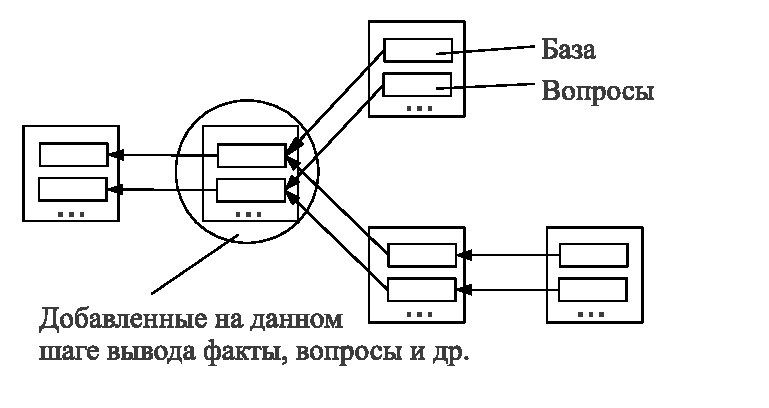
\includegraphics[width=0.6\linewidth]{pics/PST2.eps}
	\caption{ДСВ.}
	\label{fig:pst2}
\end{figure}

С точки зрения реализации ДСВ растёт от листов к корню.



%================================== СУПЕРВИЗОР =======================
\subsection{Супервизор}
Наблюдает глобально за всем деревом. Содержит информацию об ограничении ресурсов, эвристики и др.
В супервизоре находится список всех текущих листов дерева.
Большинство стратегий реализовано на уровне супервизора, поскольку иногда приходится читывать информацию о всей совокупности предшествующего или последующего вывода.

Наличие такого субъекта управления обусловлено тем что некоторые частные события в процессе логического вывода могут повлиять на него в целом.

%================================== ОГРАНИЧЕНИЕ РЕСУРСОВ =======================
\subsection{Стратегия ограниченных ресурсов.}
Стратегия ограниченных ресурсов есть в Вампире. У нас подобная стратегия напрямую зависит от текущего ДСВ и описывается так: ветка ДСВ строится до тех пор, пока не наступит ограничение разрешенной для использования памяти, либо пока не истечет определенное время, либо пока не будет произведено определенное количество шагов вывода. Если наступил предел использования ресурсов, то необходимо произвести откат назад и попробовать другие ответы, т.е. другие варианты построения дерева.

%============================================================================
%================================== РАЗДЕЛЕНИЕ ДАННЫХ =======================
\subsection{Разделение данных}
Логический вывод как правило связан с выводом новой информации. Например, в МР выводятся новые дизъюнкты до тех пор пока не выведется пустой, а в методе доказательства ПО-формул производится насыщение баз фактами до тех пор пока они не станут противоречивыми. Поскольку сложность формул может быть сколько угодно большой и даже минимальный вывод может иметь сколько угодно большую длину, имеет место быть проблема увеличения затрачиваемых ресурсов на всеразростающиеся формулы. Опыт показывает [ссылка] что автоматический вывод довольно быстро занимает всю имеющуюся в распоряжении память и далее процесс вывода требует регулярное удаление излишков. Таким образом проблема экономии памяти  довольно важна, особенно с учётом увеличения сложности задач. Для экономии памяти используются, во-первых проектирование компактных структур данных, во-вторых методы разделения общих участков памяти (data sharing). В случае логических языков и конкретно языка ПО-формул метод разделения данных довольно актуален.

Исходя из некоторых общих особенностей представления языков первого порядка и представления ПО-формул, нами выделено четыре вида разделения данных.

\paragraph{Агрессивное разделение термов.} Заключается в том, что разделяются общие участки оперативной памяти среди термов. Например, в термах $A(g(a,f(x)),h(c))$ и $B(k,g(a,f(x)))$, подтермы $g(a,f(x))$ являются общими и представляют собой один и тот же участок в памяти. Данный подход позволяет достаточно сильно экономить оперативную память при ограниченных ресурсах, однако требует дополнительное процессорное время на вычисление общих подтермов. Такой метод является общеупотребимым в системах АДТ, классически варианты реализации представлены в [].

\paragraph{Мягкое разделение термов.} Отличается от агрессивного намного большей эффективностью в смысле потребления процессорных ресурсов, но меньшей эффективностью с точки зрения экономии памяти, поскольку разделяет только часть общих подтермов. Опишем данный метод более подробно. Исходя из определения \ref{ircond} применение правила вывода $\omega$ законно в случае выполнения условия $A\theta \subseteq B$, где $A$ и $B$ соответственно конъюнкты вопроса и базы. Поскольку $B$ это уже существующее множество основных обобщенных термов, то для их хранения выделена соответствующая память. $\theta$ же является отображением переменных вопроса $A$ в элементы эрбранова универсума. В дальнейшем при применении правила вывода $\theta$ применяется ко всему консеквенту вопроса и данный консеквент добавляется к формуле. Однако правая часть подстановки уже имеется в памяти, в силу того что основана она на $B$. Исходя из этого достаточно использовать ссылки на уже имеющуюся память используемую для правых частей подстановки в тех частях консеквента где эта подстановка применяется. На рисунке детально представлена данная ситуация.

\paragraph{Разделение базовых подформул.} ПО-формулы, в которых производится ответ на вопрос имеющий вопрос с дизъюнктивным ветвлением, расщепляются на несколько новых базовых подформул. Количество новых базовых подформул совпадает с количеством непосредственных наследников в консеквенте вопроса. В прямом варианте такое расщепление требует копирования предыдущего состояния формулы несколько раз, такое копирование естественно приводит к большим затратам памяти и процессорному времени предназначеннго для копирования. Решение данного вопроса могло бы лежать в плоскости агрессивного разделения термов, однако такого разделения может быть недостаточно. Если формула предполагает достаточно сильное ветвление, сохраняется проблема наличия множества ссылок на разделяемые атомы баз. Поскольку расщепление предполагает разделение баз, то имеет смысл разделять и эти ссылки. Более подробно ситуация рассмотрена на рисунке.

Таким образом в системе кроме разделения термов используется ещё и разделение ссылок на эти термы, благодаря ДСВ.

\paragraph{Разделение переменных и неопределенных эрбрановских элементов.} Предназначено для быстрого применения подстановки ко всей формуле, т.к. все одноименные переменные в формуле представляют собой один участок в памяти. О неопределенных эрбрановских элементах сказано ниже. Все одноименные переменные на протяжении любого основного пути формулы \cite{dissChe} являются указателем на один и тот же участок в памяти. В отличие от агрессивного разделения данный подход учитывает роль переменных в процессе поиска ответных подстановок. В процессе применения подстановки переменная не заменяется на терм, а лишь указывает на этот терм, что позволяет экономить время на замену переменной термом в поддереве.

\paragraph{Веса подформул.} Кроме непосредственно экономии потребляемой памяти, реализована возможность сдерживания разрастания формулы. Для этого из возможных ответов на вопрос выбирает тот который приводит к формуле наименьшего веса. Под весом понимается количество узлов в дереве представляющем терм или формулу.


%======================== INDEXING ===========================
\subsection{Индексирование данных}

Из определения стратегии ясно, что шаг вывода зависит от некоторых \textbf{критериев}, которым должны удовлетворять определенные части ПО-формулы. Например, допустимы следующие критерии: Наличие в базе заданного терма, наличие вопроса с заданными свойствами, количество вхождений терма в конъюнкт и т.д. Для определения истинности данных критериев необходимо проводить поиск и анализ данных в формуле. С каждым шагом вывода формула в общем случае увеличивается (причем в некоторых случаях довольно сильно), и может настать момент когда поиск тех или иных данных будет затруднен.

%индексирование термов
\paragraph{Индексирование термов}

В информационных технологиях подобные проблемы разрешены с помощью методов индексирования данных (широкоприменяемых в базах данных \cite{Ulman}). Подобно тому как в библиотеке книги проиндексированы первыми буквами своих названий а также именами авторов. Такие подходы используются и в реляционных БД.

В нашем случае основной объект индексирования есть терм, который является древовидной структурой, индексирование которой в реляционных БД неэффективно [есть ссылка на это]. Поэтому следует использовать иные подходы.

Индексирование термов --- хорошо исследованный вопрос, как в рамках определенных систем АДТ, так и абстрактно. В частности по данной теме можно почитать [дискриминационное дерево и пути, подстановочное дерево, и книжку Графа про индексирование].
Перечисленные методы, позволяют эффективно находить в базе термов те термы, которые удовлетворяют определенным критериям: являются равными данному (query term), являются его примерами, обобщениями (generalization) и унификациями.
Для наших нужд не требуется обобщение и классическая унификация, но дополнительно необходимы НЭЭ Унификация, критерий наличия термов включающих заданный подтерм, и различные количественные критерии: вес, глубина, арность. С учетом перечисленных требований а также того факта, что как правило в базе находятся основные термы, мы в качестве основы выбрали методику индексирования путями [].

Кратко опишем её суть, как она описана в []. Для каждого атома составляется список так называемых путей. [Надо привести формальное определение пути из [макКьюн]]. Например, атом $A(g(x,c),e)$ представляется в виде путей $A$, $A1g$, $A1g1x$, $A1g2c$, $A2e$. Каждый из этих путей содержит указатель на соответствующей атом. Сами пути хранятся в отсортированном виде (в дереве).

Пример. Пусть дан атом $A(a,f(x,b))$ и множество атомов $\{A(a,f(c,b)), A(a,f(b,e)),A(a,f(k,b)), A(b,f(e,b))\}$. Любой атом, являющийся основным примером для заданного, содержит в своём списке путей следующие пути: $A1a$, $A2f2b$. Таким образом для поиска основных примеров заданного атома необходимо найти пересечение множеств атомов, на которые указывают пути.  В частности путь $A1a$ указывает на множество $\{A(a,f(c,b)), A(a,f(b,e)),A(a,f(k,b))\}$, а путь $A2f2b$ на $\{A(a,f(c,b)), A(a,f(k,b)), A(b,f(e,b))\}$. Пересечение этих множеств есть множество $\{A(a,f(c,b)),A(a,f(k,b))\}$, это и есть множество примеров для атома $A(a,f(x,b))$.

Заметим, что методы индексирования термов на сегодняшний день используются во многих известных системах АДТ [Vampire -улучшенное индексирование путями, Otter -дискр.дерево и пути, E, EQP, SPASS -дерево подстановок].

Кроме базы термов, в индексировании нуждаются множества вопросов и множества ответных подстановок.

%индексирование других частей фомрулы
\paragraph{Индексирование других частей формулы}
Теперь опишем иные нужды индексирования. Предположим что у нас имеется некоторая стратегия для решения некоторого класса задач. Стратегия оперирует вопросами с определенными свойствами (т.е. вопросу сопоставляется содержательная информация), которые присущи всему классу задач (т.е. все задачи объединяет наличие определенных вопросов).
Естественно было бы неплохо как-то закрепить эти вопросы что бы упростить в дальнейшем к ним доступ и каждый раз не проверять все вопросы на наличие определенного свойства.
Для этого достаточно сделать словарь (map) в котором каждому описанию вопроса соответствовал бы указатель на данный вопрос. (Конечно можно в стратегии пользоваться лишь номером вопроса, но тогда теряется гибкость, ведь пользователю необходимо будет ставить вопросы всегда на одно и тоже место.)
Данный вид индексирования (весьма простого) может выполняться как на этапе компиляции (тогда в компиляции прувера будет задействован не только стратегия но и сама задача), так и при первичном обращении к вопросу (тогда нет необходимости в компилировании самой задачи).


%================================== ЛЕНИВАЯ КОНКРЕТИЗАЦИЯ =======================
\subsection{Неограниченные переменные}
Проблема неограниченных переменных описана выше. Для её решения предложено несколько подходов.

\paragraph{Ленивая конкретизация}
Суть заключается в следующем: для открытой переменной не выбирается конкретный элемент эрбранова универсума, а в место этого она заменяется на неопределенный эрбрановский элемент (НЭЭ), который в дальнейшем исходя из нужд вывода постепенно доопределяется до основного терма, либо в некоторых ситуациях так и остается недоопределенным.
По своей природе НЭЭ схож с переменной в том смысле что он изменяем, однако все изменения касающиеся НЭЭ должны быть направлены на конкретизированные НЭЭ, т.е. НЭЭ может быть заменен либо на некий терм (возможно тоже содержащий НЭЭ) либо на другой НЭЭ, но не на переменную. Однако для переменной НЭЭ считается как терм, и можно производить замену на него.

\begin{equation}
	\forall\colon\boldsymbol{True} - \exists\colon\boldsymbol{True} -
	\left\lbrace
	\begin{array}{l}
		\forall x\colon\boldsymbol{True} - \exists\colon A(x) \\
		\forall x\colon A(f(x)) - \exists\colon B(f(x)) \\
		\forall\colon B(f(a)) - \exists\colon \boldsymbol{False}
	\end{array}\right.
\end{equation}
На первом шаге вывода имеется ответ $\{x \rightarrow h_1\}$ на первый вопрос, $x$ является неограниченной переменной, $h_1$ это неопределённый эрбрановский элемент (НЭЭ). После первого шага атом $A(h_1)$ Добавляется в базу. На втором шаге вывода имеется ответ $\{x \rightarrow h_2\}$ на второй вопрос, и $h_1$ конкретизируется до $f(h_2)$, после второго шага $B(f(h_2))$ добавляется в базу. Наконец, на третьем шаге имеется тривиальный ответ на третий вопрос и $h_2$ доопределяется до $a$.

Однако существуют особые ситуации. Рассмотрим следующий пример:
$$\fictAquantor \; - \; \exists\colon M(e) \left\{
\begin{array}{lcl}
 \forall x,y\colon M(x) & - & \exists\colon S(y),M(f(x)),T(x) \\
 \forall x \colon T(x),S(e) & - & \exists\colon Q(x) \\
 \forall x \colon Q(x),S(f(e)) & - & \exists\colon\textbf{False}
\end{array}
\right.$$

Данная формула имеет вывод, например такой: отвечаем на первый вопрос с подстановкой $\{ x\rightarrow e, y\rightarrow e \}$, в результате в базу попадают факты $S(e),M(f(e)),T(e)$; ответ на второй вопрос есть $\{ x \rightarrow e\}$ и в базу попадает $Q(e)$; полученных фактов в базе недостаточно для ответа на целевой вопрос, поэтому вновь отвечаем на первый вопрос, при этом имеет несколько вариантов ответа, но важно переменную $y$ необходимо заменить на $f(e)$, выберем, например, следующий ответ $\{x \rightarrow e, y \rightarrow f(e) \}$ и в базу попадет факт $S(f(e))$ после чего целевой вопрос имеет ответ.
Заметим что на первый вопрос необходимо обязательно выбирать те подстановки которые содержат $y \rightarrow e$ и $y \rightarrow f(e)$ необходимые для ответа на второй и третий вопросы соответственно. Также формула устроена таким образом что первый и второй вопросы всегда имеют новые ответы (надеюсь это очевидно).

Теперь рассмотрим работу стратегии отсроченного присваивания: ответ на первый вопрос будет следующего вида $\{ x\rightarrow e, y\rightarrow h_1 \}$, где $h_1$ есть НЭЭ, и в базу попадают следующие факты $S(h_1),M(f(e)),T(e)$; ответ на второй вопрос есть $\{ x\rightarrow e, h_1\rightarrow e \}$ в котором $h_1$ доопределяется до $e$ и соответственно находящийся в базе факт $S(h_1)$ доопределяется до $S(e)$; с этого момента начинается зацикливание, поскольку целевой вопрос не имеет ответа, вновь отвечаем на первый вопрос и вновь в базу попадает факт $S(h_1)$, который при ответе на второй вопрос вновь доопределится до $S(e)$ и т.д. Однако если пропустить ответ на второй вопрос, то при ответе на целевой, факт $S(h_1)$ доопределится до $S(f(e))$ и на этом вывод закончится.

В общем виде проблема заключается в том, что НЭЭ доопределяется при поиске ответов на определенный вопрос, раньше чем это необходимо при ответе на другой вопрос. То есть доопределяется там где этого уже не надо.

Из подобных примеров видно, что СОП не может использоваться на прямую. Необходимы какие-то дополнительные средства обеспечения логического вывода.

\paragraph{Первый вариант}
Одним из вариантов решения проблемы является использование языка описания стратегий, с помощью которого можно, например, указать, что на второй вопрос необходимо ответить лишь один раз, либо использовать на первый вопрос сразу несколько подстановок содержащих $y\rightarrow h_1$ и $y\rightarrow h_2$, это приведет к попаданию в базу двух фактов $S(h_1)$ и $S(h_2)$, один которых будет использоваться для второго вопроса, а другой для целевого. Такой вариант вполне приемлем и нами предполагается что именно он и будет чаще всего использоваться для решения задач. Но что делать, если дополнительные знания о задаче не позволяют сформулировать правильную стратегию? Необходимо предоставить хотя бы принципиальную возможность вывода (что пока необеспеченно).

\paragraph{Второй вариант}
Мы видим следующий путь решения данной проблемы в общем случае (т.е. без использования дополнительных стратегий): не доопределять НЭЭ на месте (как это сделано выше), а \textbf{порождать} новые выражения, полученные из исходных, заменой в них НЭЭ на доопределение. То есть если в базе содержится факт $S(h_1)$ и $h_1$ необходимо доопределить до некоторого терма $t$, то в базу добавляется новый факт $S(t)$, порожденный от $S(h_1)$, при этом сам $S(h_1)$ сохраняется. При определенных условиях также может возникнуть ситуация когда будут порождаться не только факты, но и целые подформулы.
Содержательно такой подход означает следующее: можно считать что для вопроса с открытыми переменными применяется вся совокупность возможных ответов (с использованием всех элементов эрбрановского универсума), но так как технически это нереализуемо (из-за бесконечности эрбановского универсума), используется техника ленивых вычислений. В уме мы думаем что применили все ответы, а на деле используем только необходимые.

Данный подход имеет и определенные недостатки. Связано с тем если появится вопрос с НЭЭ, то придется порождать новые вопросы, а если будет диз.ветвление, то ещё хуже. Плюс во время унификации вылазят всякие проблемы. Короче об этом надо упомянуть но сильно не выпячивать, и оправдаться тем что мы больше нацелены на использование миниязычка, а эта стратегия дана лишь для обеспечения полноты вывода. Но эта стратегия вполне эффективна если НЭЭ не будут появляться новые вопросы с НЭЭ и в диз.ветвлении их не будет...

Отметим, что стратегии основанные на использовании НЭЭ стоят особняком для многих других стратегий. Во-первых из-за этой стратегии нарушается независимость базовых подформул, поскольку один и тот же НЭЭ может быть в разных подформулах, то доопределение одного из них в одной подформуле автоматически приводит к доопределению его в другой подформуле, это в частности противоречит параллельным стратегиям и противоречит некоторым эвристическим фишкам.

\paragraph{Стратегия фильтрации эрбрановского универсума}
Ещё одним вариантом решения проблемы открытых переменных является стратегия фильтрации ЭУ. Данная стратегия позволяет избавиться от проблем вышеперечисленных, но несколько расширяет пространство возможных ответов. Суть данной стратегии заключается в следующем. Атомы консеквентов, которые (атомы) содержат неограниченные переменные вопросов, должны унифицироваться с одноимёнными атомами из всех других частей всей базовой подформулы, в противном случае атом попавший в базу не будет удовлетворять условие применения правила вывода, поскольку никода не выполнится процедура матчинга при поиске ответов. Будем использовать данное свойство в стратегии. В качестве ответа для неограниченных переменных используются основные примеры унификации. Такой подход позволяет заранее сузить пространство ЭУ, фильтруя заведомо бесполезные ответы.

Для ясности рассмотрим пример.



%======================================================================
%================================== k,m-условие =======================
\subsection{Стратегия km-условия}
Данная стратегия формулируется следующим образом. Некоторый ответ применяется, если за последующие k шагов произойдет заданное событие m раз. Пользуясь терминологией ДСВ это означает что для данного узла дерева применяется ответ в случае если построенное в результате дальнейшего вывода поддерево коренящееся с этого узла не превысит глубину k и до этого момента произойдет m раз событие.

Мы предлагаем три спецификации данной стратегии.

\textbf{km-опровержение.} Ответ выбирается в случае если за последующие k шагов будет опровергнуто m баз. Подобная стратегия первоначально предложена в \cite{ICDS2000} и реализована в КВАНТе Черкашина. В данной системе эта стратегия расширена вторым параметром m. Она позволяет сдерживать разрастание пространства поиска вывода, т.е., сдерживает излишнее ветвление ДСВ, что в некоторых случаях приводит к многократному усложнению вывода.

\textbf{km-конкретизация.} Если за последующие k шагов будет доопределено m НЭЭ. Эта стратегия также направлена на то чтоб ограничить сложность представляемой формулы. Недоопределенный НЭЭ тащит много информации за собой и много условий, что на уровне реализации влияет негативно, поэтому чем больше и быстрее НЭЭ будут доопределены нужным образом, тем лучше.

\paragraph{Особенности реализации}
Основной для реализации данной стратегии являются описанные выше ДСВ и супервизор. Параметры k,m и собственно условие закладывается в супервизоре и привязывается к определённом узлу ДСВ. Через каждый следующий шаг вывода, супервизор проверяет все условия. И в положительном случае производится откат назад, т.е. последовательное удаление узлов дерево в обратном порядке (от листа в направлении корня). Перед удалением каждого узла производится разконкретизация НЭЭ полученных на этих узлах и возврат использованных вопросов в стадию активных (т.е. возможных для применения).

%================================== КЕШИРОВАНИЕ =======================
\subsection{Кэширование результатов}
Учитывая множественность возможных ответов, откатов в выводе, большой глубины вывода, большого количества атомов в базе и т.д. целесообразно кешировать некоторые результаты чтобы не производить снова повторяющиеся вычисления.

Добавление уже имеющихся в базе атомов не допускается. Поэтому процедура поиска ответов работает всегда с новыми атомами, и производит всегда новые вычисления. Тем не менее полученные ответы в итоге могут совпадать. Все примененные ответы сохраняются, причем хранятся они как и база в чанках, размазанных по всему пути от листа до узла. Это позволяет делать корректные откаты с учетом сохранения информации о примененных ответах.

%-----------PARALLEL STRATEGY---------------------------
\subsection{Параллельные стратегии}

Полезно сполна использовать все вычислительные ресурсы. Многие современные ВС обладают бОльшим чем 1 вычислительным элементом (процессором).

Предлагаем следующие стратегии для распараллеливания процесса логического вывода.

\paragraph{Первая стратегия}

В случае если вопрос имеет дизъюнктивное ветвление, то после ответа на этот вопрос, формула расщепляется и трансформируется в формулу с б'ольшим количеством баз. Таким образом, количество базовых подформул может заметно увеличиваться. Кроме того, исходная формализация задачи в языке по-формул может содержать более одной базовой подформулы. Для того, что бы показать, что исходная формула противоречива, необходимо опровергнуть каждую из баз. Специфика исчисления ПО-формул, позволяет рассматривать данные базы независимо друг от друга (естественный ИЛИ-параллелизм, следующий из того что в базах находятся лишь основные термы), а значит, процедура опровержения каждой базы может выполняться в отдельном вычислительном процессе. Таким образом, первая стратегия, реализуемая в виде параллельной схемы алгоритмов, формулируется следующим образом: каждая базовая подформула опровергается независимо, а значит параллельно. Для нужд данной стратегии как раз и реализовано жесткое копирование (следующая глава), что бы полностью скопировать базовую подформулу и обрабатывать её в отдельном процессе независимо (не разделяя память).

\paragraph{Вторая стратегия}
Для применения каждого шага логического вывода, необходимо выполнять, в общем случае, поиск ответных подстановок для заданного вопроса. Поиск ответных подстановок не изменяет структуру формулы, и не использует общих изменяемых данных, это значит, что процессы поиска ответа на каждый вопрос независимы, а значит параллельны.


\paragraph{Третья стратегия}
Теперь рассмотрим процедуру поиска подстановок для отдельно взятого вопроса.
Как было сказано во введении, подстановка $\theta$ является ответом, если выполняется
условие $A\theta \subseteq B$, где $B$ --- конъюнкт вопроса, $A$ --- конъюнкт базы.
Для сохранения полноты необходимо хотя бы потенциально иметь в распоряжении все возможные ответы,
из которых выбирается подстановка для данного шага. Ниже описан структура хранилища ответов. Можно говорить о том что наполнение каждого чанка хранилища подстановками производится параллельно, поскольку чанки независимы.

\paragraph{Свойства стратегий}

Анализ, описанных выше стратегий, показывает, что они обладают свойством вложенности. Т.е., для того, что бы опровергнуть одну базовую подформулу (первая стратегия) необходимо найти ответы на вопросы (вторая стратегия). В свою очередь для поиска ответа, необходимо найти подстановки для каждого атома из конъюнкта вопроса (третья стратегия).

Исходя из этого, данные стратегии можно разместить по степени эффективности (иерархия стратегий). Не трудно видеть, что время, затрачиваемое на опровержение базы, как минимум, не меньше, чем время, затрачиваемое на поиск ответных подстановок, а на практике, как правило, оказывается намного больше (так как, как правило, для опровержения базы необходимо неоднократно ответить на некоторые вопросы). Аналогичные выводы делаются по отношению к другим стратегиям.

Кроме того, можно выделить единое для всех стратегий свойство – свойство однородности. Т.е. стратегии имеют единую структуру. А именно, все они, по сути, сводятся к применению некоторой операции (опровержение базы, поиск ответов и т.д.) для каждого элемента некоторого множества (базы, вопросы и т.д.).

Одной из рекомендаций при реализации описанных алгоритмов на кластерных вычислительных системах является правильное распределение задач между вычислительными узлами кластера, в зависимости от скорости коммуникации между ними. Например, программная реализация первой стратегии должна процесс привязывать к вычислительному узлу. Однако этого не стоит делать при реализации остальных стратегий, так как коммуникационные затраты, вполне вероятно, перекроют полезное время вычислений, и тем самым лишь ухудшат результат.

Отметим что данная стратегия в общем случае конфликтует со стратегией отсроченного присваивания (поскольку СОП может нарушать независимость баз и вопросов).

\paragraph{Тестирование}
Важным свойством параллельных схем алгоритмов является их масштабируемость, т.е. степень повышения эффективности с увеличением количества вычислительных элементов (ВЭ). Поэтому основной характеристикой является не конкретное время исполнения программ, а соотношение времени исполнения программы в параллельном режиме на заданном количестве ВЭ к времени исполнения этой же программы на одном ВЭ при различном количестве ВЭ.

Эксперименты проводились на задачах, формализация которых в языке ПО-формул обладает необходимыми свойствами для испытания параллельных стратегий, а именно: дизъюнктивное ветвление, большое количество вопросов, крупные конъюнкты вопроса.

Результаты находятся в соответствии с представленной иерархией стратегий. На рис. представлены результаты тестирования.

\begin{figure}[h]
	%\vspace{0.5cm}
	\centering
	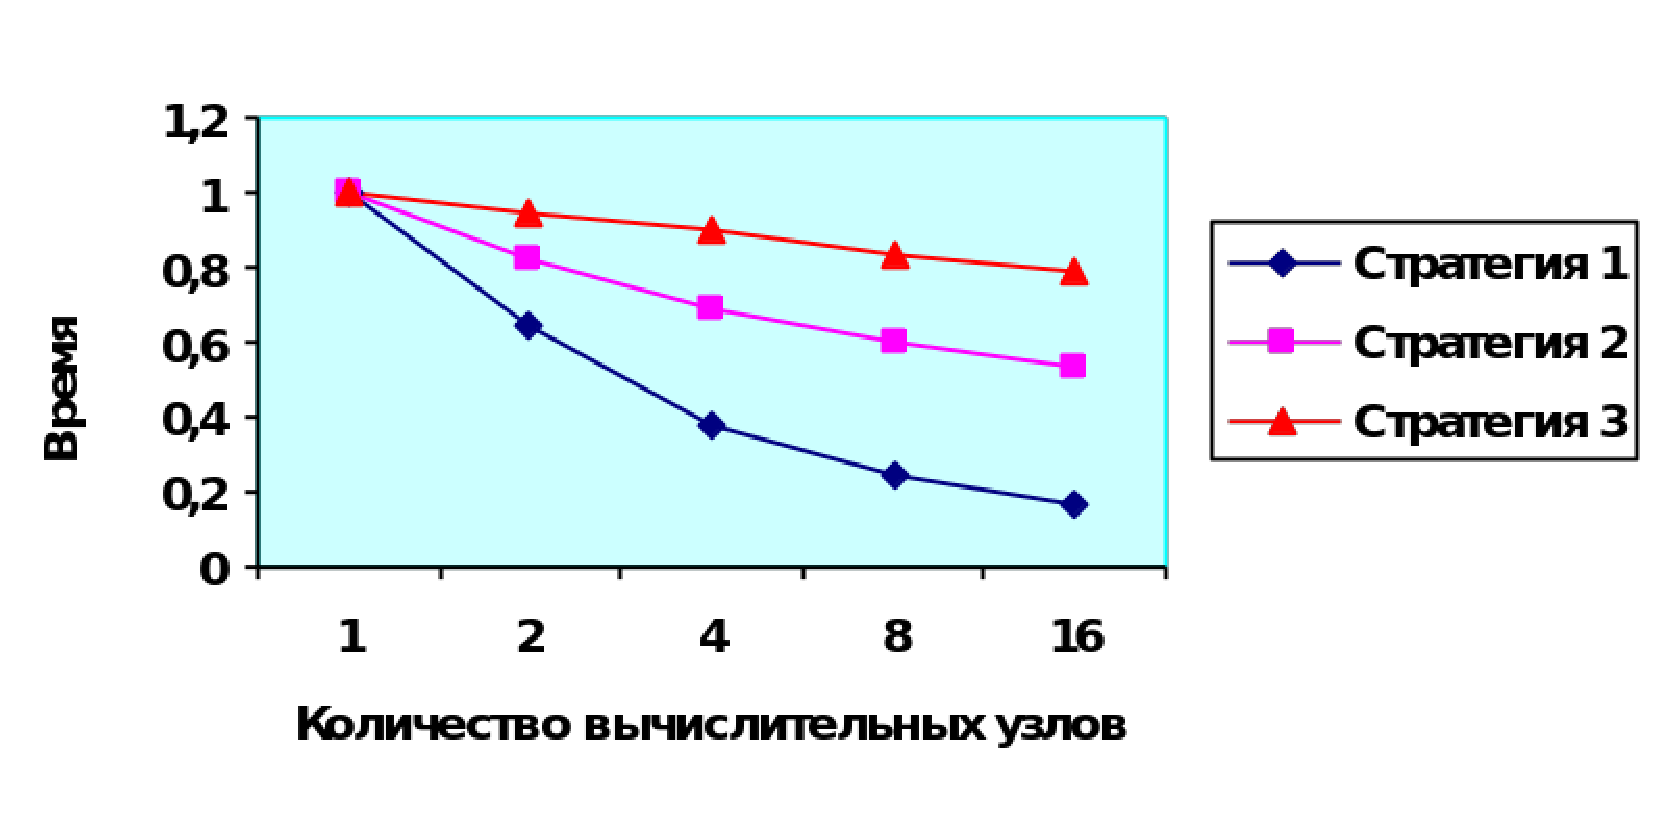
\includegraphics[width=0.6\linewidth]{pics/Parallel.eps}
	\caption{Параллельные стратегии}
	\label{fig:parallel}
\end{figure}

Наибольшую эффективность, как и следовало ожидать, показала первая стратегия (естественно при наличии дизъюнктивного ветвления). Под эффективностью понимается уменьшение затрачиваемого времени с увеличением количества вычислительных узлов.


%============================= РАВЕНСТВА =========================
\subsection{Равенства}
Для работы с равенствами как правило очень неэффективно напрямую использовать аксиомы равенства (рефлексивность, симметричность, транзитивность, подстановочность). Например, если формула содержит лишь один бинарный функциональный символ $f$ и один бинарный атомарный символ $A$, то в языке ПОФ аксиомы равенства для такой формулы будут представлены следующим образом:
$$\left\lbrace
\begin{array}{l}
\forall x\colon\boldsymbol{True} - \exists\colon x = x \\
\forall x_1,y_1,x_2,_y2\colon x_1 = y_1, x_2 = y_2 - \exists\colon f(x_1,y_1) = f(x_2, y_2) \\
\forall x_1,y_1,x_2,_y2\colon x_1 = y_1, x_2 = y_2, A(x_1,y_1) - \exists\colon A(x_2,y_2)
\end{array}\right.
$$
Таким образом, для каждого функционального и атомарного символа из формулы ставится в соответствие подформула-вопрос аксиома равенства. Явное использование таких аксиом во-первых, усложняет структуру формулы (лишние вопросы), во-вторых, увеличивает число шагов вывода, в-третьих, генерирует много (потенциально бесконечно) фактов в базе, возможно ненужных, мешающих выводу.

Отметим что данная проблема не так ужасна как в МР, поскольку в МР могут генерироваться лишние дизъюнкты, а это соответствует генерированию лишних вопросов в ПОФ. В исчислении ПОФ же генерируются лишь атомы-факты, за которыми проще наблюдать, но тем не менее их много.

При классическом подходе, в соответствии с определением ~\ref{ircond} подстановка $\theta$ является ответом на вопрос, тогда и только тогда, когда $A \theta \subseteq B$ где $A$ - конъюнкт вопроса, а $B$ - конъюнкт базы. Поиск ответов есть задача поглощения, для решения которой как правило используется алгоритм матчинга, об этом уже писалось выше. В случае ПОФ используется основной матчинг, а в случае НЭЭ используется полуосновной-матчинг.

Для решения проблемы основного матчинга без явного использования аксиом равенства имеется задача основного матчинга с равенствами, которая формулируется следующим образом [microsoft]:
Для данного множества равенств $E(B)$, основного терма $t$ и терма $p$, который может содержать переменные, необходимо найти множество подстановок $\theta$, по модулю $E(B)$, такие что $E(B)\models t = p\theta$. Через $E(B)$ мы обозначим множество всех равенств в данной базе $B$. Две подстановки эквивалентны если их правые части попарно конгруэнты по модулю $E(B)$.

Для поиска таких ответов мы используем аппарат теории систем переписывания термов \cite{Nipkow}.



%=====================================================================
%==========================ХРАНИЛИЩЕ ОТВЕТОВ==========================
\subsection{Хранилище ответов}
Хранилище ответов предназначено для эффективной организации работы с ответными подстановками и синхронизации с бэктрэкингом.

Каждому атому конъюнкта вопроса соответствует чанк возможных подстановок, матчащих этот атом с атомами из базы. Использование чанков связано с тем что необходимо точно определять на каком шаге какие подстановки были найдены. Для поиска ответа на вопрос, необходимо учитывать совокупность чанков соответствующих всем атомам конъюнкта вопроса.

На рисунке представлена схема хранения подстановок.

\begin{figure}[h]
	%\vspace{0.5cm}
	\centering
	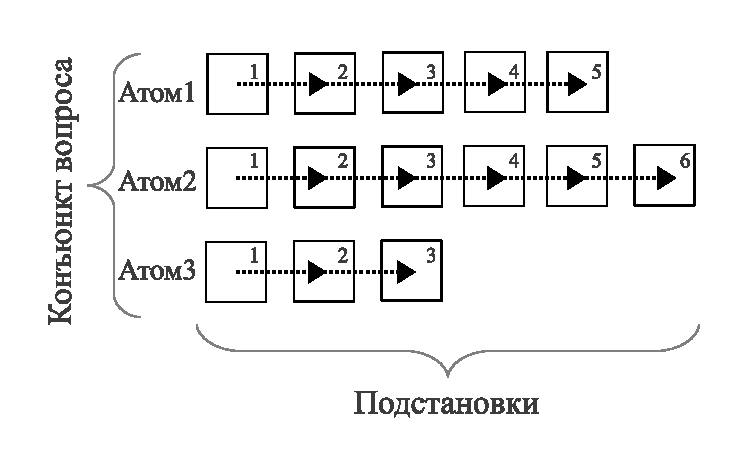
\includegraphics[width=0.6\linewidth]{pics/AnBase.eps}
	\caption{Подстановки}
	\label{fig:anbase}
\end{figure}

Далее из этой структуры выделяется ответ на вопрос. Для этого комбинируются подстановки из каждого чанка по одной. При этом подстановки должны быть совместимы. Две подстановки совместимы если их левые части равны, а правые унифицируемы. Например, если есть подстановки $\{x \rightarrow a\}$ и $\{x \rightarrow b\}$, где $b$ есть константа, то эти подстановки несовместимы, поскольку $a$ и $b$ неунифицируемы. А подстановки $\{x \rightarrow f(a)\}$ и $\{x \rightarrow f(h)\}$, где $h$ есть НЭЭ, совместимы, поскольку $f(a)$ и $f(h)$ унифицируемы с подстановкой $\{h \rightarrow a\}$. Результатом комбинации будет объединение всех совместимых и унифицирующих подстановок.

Перебор подстановок из чанков производится последовательно, это позволяет сохранить полноту.

%=================================================================================
%==================================СТАНДАРТНАЯ СТРАТЕГИЯ==========================
%=================================================================================
\subsection{Стандартная стратегия}
Главное свойство стандартной стратегии заключается в её полноте. Для полноты вывода необходимо организовать полный последовательный перебор всевозможных ответов на все вопросы. Для этого используются возможности дерева состояний вывода и хранилища ответов.


%%% Local Variables:
%%% mode: latex
%%% TeX-master: "dis"
%%% End:

% Программная система
%\chapter{Программная система}


\section{Реализация}

Программная система является системой автоматического доказательства теорем в исчислении позитивно-образованных формул. Наша система относится ко второму классу систем АДТ, согласнно классификации приведенной во введении.

%-------------------------------------------------------------------
%---------------------------------АРХИТЕКТУРА-----------------------
%-------------------------------------------------------------------
\subsection{Архитектура системы}
Картинка.


%---------------------------------------------------------------------
%---------------------------СТРУКТУРЫ ДАННЫХ--------------------------
%---------------------------------------------------------------------
\subsection{Основополагающие структуры данных и управление памятью}
%этот кусок возможно надо перенести в предыдущую главу. или наоборот.

\textbf{Подстановка.} Подстановка есть список связей (binding) вида $X \rightarrow t$. В структуре Binding для $X$ и $t$ даны имена left и right соответственно. Определены следующие методы:

apply() --- применить подставноку. В каждой связи терм left связывается с термом right, т.е. аргумент left ссылается на right. 

reset() --- сброс подстановки. Аргумент left являющийся переменной приводится в состояние NULL, а left являющийся НЭЭ не сбрасиывается. Применяется непосредственно после шага вывода, для того что бы освободить переменные для дальнейшего использования, но при этом оставить НЭЭ связанными.

fullReset() --- сброс всей подстановки, включая НЭЭ. Применяется на этапе неудачной унификации, что бы вернуть все НЭЭ в прежнее состояни


\subsection{Вспомогательные алгоритмы}

\paragraph{Копирование подформул.}
В системе реализовано два тип копирования подформул. Первый тип предназначен для корректного копирования консеквентов и перемещения их к базе. Такое перемещение должно разорвать связь между переменными и связанными с ними термами, для того что бы освободить переменную для дальнешего использования в других шагах вывода, но при этом что бы в базу попали именно те термы с которыми данная переменная связана. Кроме того такой тип копирования нужен для параллельных стратегий, что бы переместить формулу в полностью независимый процесс. Данный тип копирования будем назвать жестким.

Второй тип копирования предназначен для правильной обработки НЭЭ с учетом бэктрэкингда. Поскольку при откатах необходимо востсанавливать информацию о том какой НЭЭ был связан с каким термом. Копирование НЭЭ проводится в прямую, вместе с привязанным к нему термом. Но потом такой НЭЭ в базе идентифицируется как связанный и работа ведется с привязанным термом. Такой тип копирования будем называть мягким.


\paragraph{Матчинг с НЭЭ.} В сисеме реализован классический алгоритм матчинга адаптированный для случая содержания в термах НЭЭ. Для матчихщася термов строятся уравнения. Поведение НЭЭ определяется следующим образом. Если в уравнении НЭЭ находится в првой части, то его поведение совпадает с поведением универсальной переменной. Если слева, то НЭЭ не может быть доопределён до другой переменной. Если и справа и слева находятся НЭЭ, то возникает два варианта развития. Либо они совпадают и оба доопределяются до общего НЭЭ, либо несовпадают и алгоритм матчинга заканчивается неудачей. 

\paragraph{Выбор вопроса.}

\paragraph{Трансформация формул.} Удаление фиктивынх кванторов. Расширение или углубление формулы.

\paragraph{Проверка доказательства.} Имеется протокол вывода. Проверяется его корректность.

%====================================================================
%======================== СИСТЕМНЫЕ ПРЕДИКАТЫ =======================
%====================================================================
\subsection{Системные предикаты и вычислимые термы}
В логических языках программирования, например, Прологе \cite{Bratko}, введены так называемые системные предикаты (встроенные предикаты, built-in predicates), особенность которых заключается в том, что они или выполняют некоторое побочное действие, например, вывод на экран, чтение файла и др., или их истинность вычисляется из значений параметров, например, var(X) в Прологе определяет, является ли терм X переменной. 
В данной работе рассматривается использование системных предикатов для управления логическим выводом в процессе построения автоматического доказательства теорем в исчислении ПО-формул, то есть как способ задания дополнительных знаний о задаче в виде модификаторов стратегии, используемой по умолчанию.

Будем называть системным предикатом такой предикат, атомы которого входят в конъюнкты дерева ПО-формулы, но не участвуют непосредственно в ЛВ. Системные предикаты не имеют прямого отношения к формализации задачи, однако влияют на процесс ЛВ некоторыми побочными действиям, их истинностные значения вычисляются, выводят некоторую системную информацию. В языках логического программирования, например, Прологе, системные предикаты служат, в основном, для исполнения некоторых интерактивных действий: вывод информации на экран, чтение и запись файла, добавление и удаление фактов и др. 
Введем следующие системные предикаты:
Next(L). Переход к вопросу, помеченному идентификатором L. Предикат помещается в коньюнкт корневой вершины консенквента вопроса.  Если на данный вопрос будет произведен ответ, то следующим вопросом, для которого будет производится выбор ответа, будет вопрос (множество вопросов), помеченный идентификатором L. Таким образом, при помощи данного предиката задаются варианты порядка ответа на вопрос.

OffQuestion(L)/OnQuestion(L). Отключение/включение вопроса с идентификатором L. Отключенный вопрос объявляется неактивным, то есть не принимает участие в логическом выводе, при этом в любой момент может быть заново включен.

RemQuestion(L). Удаление вопроса с идентификатором L. 

RemFact(L) и RemPatternFact(L). Удаление факта помеченного идентификатором L, а также удаление всех основных примеров L, в случае если L – терм. 

OffFact(L)/OnFact(L). Отключение и включение факта с именем L. Поведение подобно включению и отключению вопросов.

Write(T). Печать терма T.

Save(L). Пометить состояние процесса поиска ЛВ в данной базовой подформуле идентификатором L.

Rollback(L). Откатить (backtrack) состояние вывода в базовой подформуле до состояния L с утерей более поздних по отношению к L маркировок.

Commit(L). Фиксировать состояние базы L как неоткатываемое, при этом фиксируются все состояния, помеченные ранее, чем L. 

Предикаты Commit и Rollback без параметров фиксируют или откатывают последнюю метку.
Для пометки выражений используется следующий синтаксис E’(L), где E – выражение, L – метка.
Кроме того, вводятся арифметические операции, используемые в конъюнкте вопроса и вычисляющие свои аргументы. Если арифметическая операция выполняется над полученными в подстановке аргументами, то подстановка используется в шаге вывода, иначе данная подстановка отвергается.
Рассмотрим некоторые ситуации, при которых перечисленные выше предикаты можно использовать и получать новые свойства процесса поиска ЛВ.

\textbf{Ключевые точки в доказательстве.} Нередко бывает так, что заранее известна некоторая точка, через которую должно пройти доказательство. Достаточно простым примером может служить задача поиска пути в городе между двумя точками, находящимися на разных берегах реки, при наличии одного моста. Понятно, что любой путь будет проходить через мост, однако заранее неизвестно как именно строится этот путь. Предположим, что первая группа вопросов отвечает за правила движения в первой половине города, а вторая за движение во второй половине. Очевидно, что нет смысла пытаться отвечать на вопросы второй группы, пока не преодолен мост, а после его преодоления нет смысла отвечать на вопросы первой группы. Таким образом, перед началом доказательства, вопросы второй группы объявляются неактивными, а после ответа на специальный вопрос описывающий факт перехода через мост, неактивными объявляются вопросы первой группы, а вопросы второй группы включаются. 

\textbf{Очищение формулы.} Другим типом задач являются задачи с некоторой дискретизацией шагов. Например, если моделируется переход системы из одного состояния в другое во времени, шаг такого перехода может быть эквивалентен нескольким шагам правила вывода . Часть выведенной информации, отвечающая за сам процесс перехода, может быть удалена, а другая часть, отвечающая за описание нового состояния, сохраняется. Примером может служить задача планирования движения робота в дискретном пространстве. Часть информации устаревает, и ее необходимо регулярно удалять из базы. Кроме того, устаревать могут и вопросы, отвечающие за конструктивные средства описания перехода из одного состояния в другое (движение ноги, кабины лифта и др.). Например, в базе должна оставаться история пройденного пути или решения поставленных роботу задач (обслужить все вызовы и т.п.). 

\textbf{Улучшение эффективности вывода.} Рассмотрим простую задачу вычисления n-ого элемента ряда Фибоначчи. На языке ПО-формул данная задача вычисления 10-ого элемента ряда формализуется следующим образом:

\begin{equation}
	\forall\colon\boldsymbol{True} - \exists\colon f(1,1), f(2,2) - 
	\left\lbrace
	\begin{array}{l}
		\forall n,x,y\colon f(n,x),f(n+1,y) - \exists\colon f(n+2,x+y) \\
		\forall x\colon f(10,x) - \exists\colon \boldsymbol{False} 
	\end{array}\right.
\end{equation}

где в процессе поиска подстановки $\theta$ операция «+» из значений ее аргументов вычисляется в константу (целое число), данная константа используется в $\theta$ вместо операции «+»; в консеквенте вопроса операция «+» заменяется на вычисленную константу во время применения подстановки.

В ходе ЛВ, база постепенно наполнится фактами и станет возможным ответ на целевой вопрос. При обычном выводе, с каждым ответом на первый вопрос в базу помещаются ответы, некоторые из которых будут дублироваться и как следствие могут производиться излишние вычисления. Вычисления ряда Фибоначчи подразумевает, что для вычисления последующего элемента достаточно использовать лишь два предыдущих элемента ряда. Это значит, что базу можно ограничить двумя последними добавленными элементами. Поскольку ответ на первый вопрос приводит к добавлению базы только одного нового факта, базу можно ограничить с помощью ввода системного предиката, удаляющего один самый старый элемент базы. Первый вопрос ПО-формулы с системным предикатом будет выглядеть так:
\begin{equation}
	\forall n,x,y\colon f(n,x),f(n+1,y) - \exists\colon f(n+2,x+y)'(n+2), remFact(n)
\end{equation}

при этом запись $'(L)$ означает «пометить терм меткой L». Соответственно база данной ПО-формулы выглядит так:
\begin{equation}
\exists\colon f(1,1)'1, f(2,2)'2  
\end{equation}

Удаление элементов из базы можно организовать без использования меток атомов, если использовать RemPatternFact:
\begin{equation}
	\forall n,x,y\colon f(n,x),f(n+1,y) - \exists\colon f(n+2,x+y)'(n+2), remPatternFact(f(n,_))
\end{equation}

Символ подчеркивания интерпретируется как и в Прологе в качестве анонимной переменной. Из базы будут удалены все факты, являющиеся основными примерами  $f(n,_)$. Нетрудно заметить, что такой подход эквивалентен предыдущему, однако не требует дополнительных меток атомов.

\textbf{Косвенное управление.} Вывод (в смысле, ввод/вывод данных) некоторой системной информации, косвенно можно отнести к управлению логическим выводом. Поскольку данная информация может интерпретироваться пользователем или возможно иной программой управления ЛВ, как некоторые входные данные для принятия решения. Среди выводимой информации отметим следующие: текущий шаг вывода, имя базы, имя вопроса, ответная подстановка, количество фактов в базе, количество опровергнутых баз, количество вопросов, количество потенциальных ответов, время ЛВ и печать некоторых термов.

\paragraph{Вычислимые термы.} При решении прикладных задач может быть что заранее известна семантика формулы, область интерпретации и т.д. Отсюда некоторые сложные термы можно просто вычислять, а не выводить классическим образом, или как в случае с равенствами не использовать апарат перписывания термов или кодированых деревьев. Для этого каждому символу сигнатуры должна быть поставлена в соответствие некоторая функция.

Для обобщенного терма реализован метод GTerm reduce() вычисляющий его значение. Вычисление допустимо если всего его аргументы являются также вычислимыми термами, а все переменные и НЭЭ связаны. В соответсвии со строковым представлением символа, ему задаётся его семантика в виде лямбда выражения.


%------всякие дополнительные плюшки
\section{Язык и трансляторы формул} 

\subsection{Язык формул для прувера}
БНФ?

\subsection{Транслятор из формул ИП в ПО-формулы}
Алгоритм трансляции. 

\subsection{Транслятор из TPTP в ПО-формулы}
Для представления формул на языке предикатов первого порядка используется формат представления формул библиотеки TPTP.

\section{Интерпретация полученных результатов}
С каждым узлом ДСВ связывается некоторе событие (сообщение). В каждый момент времени по текущену состоянию ДСВ можно интерпретировать что же произошло, путём последовательного вывода сообщений начиная от корня и заканчивая листом, для каждой базы.


%-----------интерактивные возможности
\section{Интерактивные возможности}
Например, при решении задачи о лифтах надо как-то добавлять информацию о поступающих выводах извне.

Как-то надо совместить это с Миниязычком.

%========================= КОММЕНТАРИИ ====================
\section{Комментарии по предложенным стратегиям}
Анализ методик показывает, что структура вывода --- ДСВ тем более эффективна и тем выше её КПД чем больше элементов может содержаться в чанках. Размер чанка зависит от соответствующих консеквентов формулы. В терминах языка ПО-формул, более предпочтительными являются формулы имеющие как можно более крупные конъюнкты, и формулы имеющие глубину. Анализ задач из библиотеки TPTP показал что такой-то класс задач при формализации в языке ПОФ обладает описанным свойством.

При классическом подходе поскольку должны быть опровергнуты все базы, не стоит пытаться опровергать их одновременно, разростая тем самым дерево, можно сэкономить память строя однобокое дерево и доказывая всегда одну ветвь, таким подходом можно увеличить глубину пространства поиска.


%-----------------------------------------------------------------------------------------
%---------------------Интерфейс------------------------------------------------
%-----------------------------------------------------------------------------------------
\section{Интерфейс и спецификация}




%%% Local Variables: 
%%% mode: latex
%%% TeX-master: "dis"
%%% End: 


% Применение
%\chapter{Применение программной системы}
\label{part:examples}

В данной главе продемонстрированы примеры применения разработанных инструментальных средств  для решения практических задач. В частности, рассматривается пример 

%-----------------------------------------------------------------------------------------
%---------------------Эксперименты, тестирование, сравнение------------------------------
%-----------------------------------------------------------------------------------------
\section{Применимость}
Как видно, каждый узел дерева состояний вывода олицетворяет шаг вывода. Кроме того, узел содержит очень много дополнительной информации, т.е. потребляет ресурсы памяти, причем с каждым шагом вывода потребление может увеличиваться. Таким образом с точки зрения потребляемости ресурсов прувер эффективнее использовать на задачах имеющих крупноблочную структуру, т.е., при формализации конъюнкты действительно должны быть конъюнктами а вырожденными одноэлементными или пустыми, древовидная структура действительно должна быть древовидной, глубокой, а не с глубиной 4. Таким образуом получится что каждый узел будет “обслуживать” довольно объемные и информативные куски данных. Одновременно с этим язык ПО-формул как раз и позиционируется как крупноблочный. Отсюда предположительно успех может возникнуть в задачах, формализуемых в языке ПО-формул таким образом, чтоб как можно сильнее выпячивалась крупноблочность. В самой крупной библиотеке формализованных задач из 10000 задач оказалось что 2000 обладают этим свойством. Поэтому тестирование и сравнение будет проводиться в следующих выборках: задачи которые предположительно наиболее удачно подходят для нашего прувера; и задачи которые предположительно являются неподходящими. 

С другой стороны задачи с неограниченными переменными приводят к использования стратегии ленивой конкретизации, что в конечном итоге может усложнить прозрачность логического вывода. Отсюда к перечисленным выше выборкам будут добавлены задачи с ограниченным и неограниченными переменными.

%=============================== ТЕСТИРОВАНИЕ И СРАВНЕНИЕ======================
\section{Тестирование}

Тестирование системы проводилось на задачах из библиотеки TPTP (www.tptp.org). Данная библиотка является де-факто стандартом для тестирования систем АДТ. На момент написания работы библиотека содержала свыше 20000 задч, формализованных на языке предикатов первого порядка (FOF: first-order formula), конъюнктивной нормальной формы (CNF: conjunctive normal form), TFF.

Все задачи классифицированы по некоторым параметрам, а именно:
\begin{enumerate}
\item Рейтинг. Измеряется числом от 0.0 до 1.0. Задача с рейтингом 0 может быть решена любым прувером внесённым в библиотеку. Задача с рейтингом 1.0 ещё не была решена ниодной системой. Задачи с рейтингом выше 0.5 считаются весьма сложными. Тестирование имеет смысл проводить по всем видам рейтинга от 0.0 до 1.0.
\item Предметная область задачи. Например, теоремы математического анализа, алгебры, геометрии, головоломки.
\item Количественные характеристики формулы. Например, количество предикатов, функциональных символов, наличие предиката равенства, общий объем формулы.
\end{enumerate}



\section{Конкретные задачи}

\subsection{Задачи без неограниченных переменных}
Из решенных задач время быстрее чем у Otter. Оттер выводит системную инфу всякую, поэтому думаю сопоставимо время на самом деле.

Задача; Рейтинг; Статус (Решил ли прувер); Комментарий.

ALG211+1; 0.12; Теорема (Да); 0.05 и 40 шагов.

MGT001; 0.12; Теорема (Да); 0.03с и 33 шага.

MGT008; 0.12; Теорема (Да); 0.007с и 6 шагов.

MGT010; 0.08; Теорема (Да); 0.007с и 13 шагов.*

MGT015; 0.12; Теорема (Да); 0.1с и 7 шагов.

MGT007; 0.12; Теорема (Да); 0.01с и 25 шагов, есть ветвление.

GRA014; 0.00; Теорема (Да); 1.2с и 5201 шагов. У Otter уходит 7 секунд. При этом вывод системной инфы не такой огромный.

GEO175+1; 0.12; Теорема (Да); 0.01 и 19 шагов.

GEO175+2; 0.12; Теорема (Да);

GEO177+1; 0.25; Теорема (Да); 0.01 и 41 шаг.

GEO178+1; 0.04; Теорема (Да); 0.01 и 42 шага.

GEO179+1; 0.08; как обычно

GEO180+1; 0.21;

GEO180+2; 0.17;

GEO183+1; 0.08; ; 28 шагов.

GEO184+1; 0.08; ; 9 шагов.

GEO186+1; 0.12;

GEO187+1; 0.21;

GEO188+1; 0.17;

GEO189+1; 0.25;

GEO190+1; 0.21;

GEO195+1; 0.29;

194+1, 193+1, 197+1, 198+1, 200+1, 201+1, 202+1, 203+1, 204-216, 236,   

SET913+1; 0.04; ..







%%% Local Variables: 
%%% mode: latex
%%% TeX-master: "dis"
%%% End: 

% Заключение
%\chapter*{Заключение}

%Общая характеристика полученных в диссертации результатов.
В диссертации представлены результаты исследования исчисления ПО-формул, как формализма для автоматического доказательства теорем (АДТ). Основным результатом является программная система АДТ, в которой реализован ряд стратегий повышающих эффективность логического вывода. Среди предложенных и реалиозованных стратегий имеются как адаптированные из других методов для ПО--формул, так и оригинальные. 

Разработанный вид системы АДТ (пруверов) занимает промежуточное положение между интерактивными системами и классическими, позволя с одной строны производить достаточно автоматизированный логический вывод, с другой стороны вовлекать в процесс человека, тем самым используя основной дубль свойств человеко- и машинно-ориентированность.

Любые исследования в данной области являются актуальными. Формальное доказательство теоремы может иметь сколь угодно большую минимальную длину, поэтому любые методы позволяющие сократить число шагов вывода, а так же скорость их проведения важны. Многие современные и самые производительные системы АДТ уже столкнулись с проблемой сложности расширения и использования дополнительных знаний о задаче (универсализм систем). Данная работа является реализацией одного из способо решения этих проблем.


% Выносимые на защиту результаты.
В рамках диссертации получены и на защиту выносятся следующие результаты:
\begin{enumerate}
\item Адаптированны некоторые общеупотребимые стратегии. Три типа параллельных стратегий, индексирование термов, один вариант разделения памяти (data sharing).
\item Реализованы оригинальные стратегии предложенные именно для исчисления ПО-формул. Дерево состояний вывода, $k,m$--ограничение, стратегии напарвленыные на решение проблем открытых переменных, варианты разделения памяти.
\item Реализован транслятор формул из языка библиотеки TPTP в язык ПО--формул.
\item Показана хорошая производительнсть системы на задачах из библиотетки TPTP.
\end{enumerate}

%\begin{enumerate}
%\item Исследование языка и исчисления ПО--формул, анализ его свойств, влияющих на возможность адаптации существующих алгоритмов и разработки новых алгоритмов;
%\item Разработка эффективных структур данных представления ПО--формул в памяти компьютера;
%\item Разработка алгоритмов преобразования ПО--формул для организации автоматического логического ввода;
%\item Адаптация существующих методик реализации алгоритмов АДТ для исчисления ПО--формул;
%\item Исследование вопросов автоматизации построения эффективного логического вывода с использованием предиката равенства;
%\item Разработка программной системы АДТ, создание инструментальных средств для программирования специальных версий АДТ, ориентированных на определенные классы теоретических и практических задач поиска ЛВ.
%\item Апробация разработанных программных средств в решении тестовых и практических задач.
%\end{enumerate}

% Достигнута ли цель диссертации?
В диссертации показана возможность использования разработанных инструментальных средств при создании программных систем.

%Конструктивная [само]критика результатов диссертации.
Несмотря на то, что в диссертации получен ряд положительных результато, необходимо сделать следующие замечания.

Основными особенностями, препятствующими внедрению разработанных инструментальных средств, на наш взгляд, являются:

\begin{enumerate}
\item Условие достаточно хорошего понимания принципов логического программирования и особенностей формализма ПО--формул у пользователя;
\item Проблема равенств решена не так эффективно, как в иных системах АДТ. %Универсальная слабость прувера. То есть система показывает себя не достаточно сильно при решении задач без  использования эвристик и модификаторов семантик. 
\end{enumerate}

Проблема 1 может быть частично или полностью решена путём развития пользовательских интерфейсов и путем просвящения пользователей. Проблема 2 требует дальнейшего отдельного исследования.

%На проблему 2 стоит смотреть с точки зрения области применения систем. То есть не использовать систему там где необходимо решать универсальным методом, и использовать там где возможно использование сильных сторон исчисления ПО-формул.

% Направления дальнейших исследований и развития в целом.

Перспективы развития естественным образом делятся на два класса: развитие фундаментальной части (языка и исчисления ПО--формул), в частности исследования вопросов построения модальных исчислений, дескриптивных, высшего порядка; и непосрдественно расширение класса решаемых задач, в частности применение в области семантического веба (как достаточно хорошо развивающегося направления), биоинформатики.

Дальнейшая разработка системы связана с продолжнием повышения производительности поиска ЛВ.


%%% Local Variables: 
%%% mode: latex
%%% TeX-master: "dis"
%%% End: 


%\protect\printbibliography
%\begin{thebibliography}{99}

%\bibliography{intelle}
%\bibliographystyle{unsrtre}

\bibitem{Bratko} Братко И. Алгоритмы искусственного интеллекта на языке PROLOG / Издательство Вильямс. 2004. 640с.

\bibitem{Butakov1} Бутаков М.И., Курганский В.И. О решении задачи трансляции планированием вычислений на основе позитивно--образованных формул // Системы управления и информационные технологии. 2007. c.~120-123.

\bibitem{ICDS2000} Васильев С.Н. Интеллектное управление динамическими системами. / Васильев С.Н., Жерлов А.К., Федунов Е.А., Федосов Б.Е.  M.:Физматлит, 2000.

\bibitem{Vas1995} Васильев С.Н. Об исчислениях типово-кванторных формул / Васильев С.Н., Жерлов А.К.  // ДАН, Т.~343, N~5, 1995, с.~583---585.

\bibitem{GilbertAkkerman} Гильберт Д., Аккерман В. Основы теоретической логики. Государственное издательство иностранной литературы. 1947.

\bibitem{Gulamov} Гулямов Ш.Б. Математическое и программное обеспечение решения первопорядковых логических уравнений. канд. дисс. текст. ИДСТУ СО РАН, Иркутск, 1997. 155~С.

\bibitem{yodan} Йодан Э. Структурное проектирование и конструирование программ. 1979. 415с.

\bibitem{QUANT4} Ларионов А.А., Терехин И.Н., Черкашин Е.А., Давыдов А.В.
Программная система КВАНТ/4 для автоматического доказательства теорем
// Труды ИМЭИ ИГУ. Математика и информатика : сб.научных трудов / под
ред.: Ю. Д. Корольков [и др.]. - Иркутск : Изд-во ИГУ, 2011. - Выпуск
1 с. 77-85.

\bibitem{LogicComp} Макаров И.М., и др. Логика и компьютер. Выпуск 5. 2004.

\bibitem{Maslov_1964} Маслов С. Ю. Обратный метод установления выводимости в классическом исчислении предикатов. / Маслов С. Ю. // ДАН СССР, Т.~159, N.~1. 1964. С.~17---20.

\bibitem{NNN} Непейвода Н.Н. Прикладная логика / Издательство Новосибирского Университета. 2000. 524c.

\bibitem{ChenLi} Чень Ч., Ли Р. Математическая логика и автоматическое доказательство теорем. 1983. 360c.

\bibitem{dissChe} Черкашин Е.А. Программная система КВАНТ/1 для автоматического доказательства теорем. канд. дисс. текст. / Черкашин Е.А. / ИДСТУ СО РАН, Иркутск, 1999. 155~С.

\bibitem{Che2} Черкашин Е.А. Разделяемые структуры данных в системе автоматического доказательства теорем КВАНТ/3. / Черкашин Е.А. // Вычислительные технологии. 2008. Т.~13. С.~102---107.

\bibitem{Church1} Чёрч А. Введение в математическую логику. Том 1. 1956 г.




\bibitem{DPL2} Alexandrescu A. The D Programming Language. / Addison-Wesley Professional; 1 edition, June 12, 2010

\bibitem{ATP_DB} Aravindan C., Baumgartner P. Theorem Proving Techniques for View Deletion in Databases // Journal of Symbolic Computation - Special issue on advances in first-order theorem proving. Volume 29 Issue 2, Feb. 2000. pp.~119---147.

\bibitem{erlang} Armstrong J. Programming Erlang. The Pragmatic Programmers. 2007.

\bibitem{Nipkow} Baader, F., Nipkow, T.: Term Rewriting and All That. Cambridge University Press, Cambridge. 1988.

\bibitem{KBAlg} Bachmair L., Dershowitz N., Plaisted D. A. Completion without failure. 1989.

\bibitem{SourceLCL} Balsiger P., Heuerding A., Schwendimann S. A Benchmark Method for the Propositional Modal Logics K, KT, S4 // Journal of Automated Reasoning Volume 24, Number 3 (2000), 297-317.

\bibitem{ProblemOrientedATP1} Bibel W., Korn D., Kreitz C., Schmitt S. Problem-Oriented Applications of Automated Theorem Proving // Design and Implementation of Symbolic Computation Systems. International Symposium, DISCO '96 Karlsruhe, Germany, September 18–20, 1996. pp.~1---21.

\bibitem{ATP_NLP} Blackburn P. Automated Theorem Proving for Natural Language Processing

\bibitem{ATP_Vision} Bondyfalat D., Mourrain B., Papadopoulo T. An Application of Automatic Theorem Proving in Computer vision // Automated Deduction in Geometry. Second International Workshop, ADG’98 Beijing, China, August 1–3, 1998. pp. 207---232.

\bibitem{Bourbaki} Bourbaki N.. Theory of Sets. Paris, Hermann. 1968.

\bibitem{protolan} Brak R.L., Fleuriot, J.D., McGinnis, J. Theorem proving for protocol languages // In: The Second European Workshop on Multi-Agent Systems, Barcelona, Spain. 2004.

\bibitem{Vassilyev_1997} Butyrin S. A., Makarov V. P., Mukumov R. R., Somov Ye., Vassilyev S. N. An {E}xpert {S}ystem for {D}esign of {S}pacecraft  {A}ltitude {C}ontrol {S}ystem // Artificial Intelligence in Engineering. V.~11(1). 1997. P.~49---59.

\bibitem{chellas} Chellas B.F. Modal Logic: An Introduction / Cambridge University Press. February 29, 1980. 312p.

\bibitem{hardver} Claessen K., Hähnle R., Mårtensson J. Verification of Hardware Systems with First-Order Logic // 

\bibitem{ATP_Flow} Darvas Á., Hähnle R., Sands D. A Theorem Proving Approach to Analysis of Secure Information Flow // SPC'05 Proceedings of the Second international conference on Security in Pervasive Computing. pp.~193---209.

\bibitem{Frege} Frege G. Begriffsschrift: eine der arithmetischen nachgebildete Formelsprache des reinen Denkens. Halle, 1879.

\bibitem{Ulman} Garcia-Molina H., Ullman J. D., Widom J. Database Systems: The Complete Book / Prentice Hall. 2009. 1210p.

\bibitem{Godel1929} Godel K. Über die Vollständigkeit des Logikkalküls. Doctoral dissertation. 1929.

\bibitem{subtree} Graf P. Substitution Tree Indexing // Proceedings of the 6th International Conference on Rewriting Techniques and Applications. 1995. P.~117---131.

\bibitem{TermIndexingBook} Graf P. Term Indexing (Lecture Notes in Computer Science / Lecture Notes in Artificial Intelligence). Springer; 1 edition. March 27, 1996.

\bibitem{PracticalLogic} Harrison J. Handbook of Practical Logic and Automated Reasoning. Cambridge University Press; 1 edition. April 13, 2009.


\bibitem{SourceBook} Heijenoort J. From Frege to Gödel: A Source Book in Mathematical Logic, 1879-1931, 1967 (1999).

\bibitem{med1} Hommersom A.J., Lucas P.J.F., Bommel P. Automated Theorem Proving for Quality-checking Medical Guidelines // CADE-20 : 20th International Conference on Automated Deduction, Tallinn, Estonia, July 22-27, 2005 : Workshop on Empirically Successful Classical Automated Reasoning (ESCAR).


\bibitem{ATP_geometry} Kortenkamp U., Richter-Gebert J. Using Automatic Theorem Proving to Improve the Usability of Geometry Software // In Proceedings of the Mathematical User Interfaces Workshop. 2004.


\bibitem{PSETHEO}  Letz R., Stenz G., Wolf A. P-SETHEO: Strategy Parallel Automated Theorem Proving // Proceedings of the International Conference on Automated Reasoning with Analytic Tableaux and Related Methods (TABLEAUX-98). 1988.

\bibitem{ATP_Ver2} Maus S., Moskal M., Schulte W. Vx86: x86 Assembler Simulated in C Powered by Automated Theorem Proving // Algebraic Methodology and Software Technology. 12th International Conference, AMAST 2008 Urbana, IL, USA, July 28-31, 2008. pp.~284---298.

\bibitem{disctree} McCune W. Experiments with Discrimination-Tree indexing and Path Indexing for Term Retrieval // Journal of Automated Reasoning. 1992. V.~9(2). P.~147-167.

\bibitem{McCuneRob} McCune W. Solution of the Robbins Problem // Journal of Automated Reasoning, V.~19(3), p.~263---276, December 1997.

\bibitem{microsoft} Moura, L., Bjorner, N. Efficient E-matching for SMT Solvers. Proceedings of th 21st international conference on Automated Deduction: Automated Deduction, Bremen, Germany July 17--20, 2007) 167--182.

\bibitem{Newell1} Newell A., Shaw J.C. Programming the Logic Theory Machine // In Proceedings of the 1957 Western Joint Computer Conference, IRE, 1957, P.230---240.

\bibitem{Newell2} Newell A., Shaw J.C., Simon H.A. Empirical Exploration With the Logic Theory Machine // Proceedings of the Western Joint Computer Conference, Vol. 15, 1957, P.218---239.

\bibitem{constrgeo} Plato J. A Constructive Theory of Ordered Affine Geometry // Indagationes Mathematicae. Volume 9, Issue 4, 21 December 1998. pp.~549---562

\bibitem{promsy} Promsky A.V. Towards C-light Program Verification: Overcoming the Obstacles // Proc. International Workshop on Program Understanding, 19-23 June, Altai Mountains, Russia, 2009. pp.~53---63.

\bibitem{Ryazanov2003} Riazanov A. Implementing an Efficient Theorem Prover /  PhD thesis, The University of Manchester, 2003. 216~P.

\bibitem{Robinson_1965} Robinson J. A. A Machine--Oriented Logic Based on the Resolution Principle. / Robinson J. A. //  Journal of the ACM. (12). 1965. P.~23---41.

\bibitem{Eprover} Schulz S. E --- A Brainiac Theorem Prover // AI Communications - CASC. Volume 15 Issue 2,3, August 2002. pp.~111---126.

\bibitem{HARIndex} Sekar R., Ramakrishnan I.V., Voronkov A. Term Indexing. In: Robinson, A., Voronkov, A. (eds.) Handbook of Automated Reasoning, pp. 1853--1964. MIT Press, Cambridge. 2001.

\bibitem{Sourcebook} Smith D.E. A Source Book in Mathematics. 1984.

\bibitem{progress19972001} Sutcliffe G., Fuchs M., Suttner C. Progress in Automated Theorem Proving, 1997-1999 // Workshop on Empirical Methods in Artificial Intelligence, 17th International Joint Conference on Artificial Intelligence, (Seattle, USA), 2001. 53---60.

\bibitem{BTPStickel} Stikel M.E. Building theorem provers // Automated Deduction – CADE-22. 22nd International Conference on Automated Deduction, Montreal, Canada, August 2-7, 2009. pp.~306---321.

\bibitem{pathindex} Stickel M. The path-indexing method for indexing terms // Technical Note 473, Artificial Intelligence Center, SRI International, RAVENSWOOD AVE., MENLO PARK, CA 94025

\bibitem{semweb} Tammet T. Extending Classical Theorem Proving for the Semantic Web // In R. Volz, S. Decker, I. Cruz, editors, Proceedings of the First International Workshop on Practical and Scalable Semantic Systems, October 2003.

\bibitem{SNV1990} Vassilyev, S.N. Machine Synthesis of Mathematical Theorems. The Journal of Logic programming, V.9, No.2--3, 1990. pp. 235---266

\bibitem{WangHao} Wang H. Toward Mechanical Mathematics // IBM J. Res. Devel., Vol. 4, No 1, 1960, P. 2---22.

\bibitem{SPASS} Weidenbach C., Dimova D., Fietzke A., Kumar R., Suda M., Wischnewski P. SPASS Version 3.5 // Automated Deduction – CADE-22. 22nd International Conference on Automated Deduction, Montreal, Canada, August 2-7, 2009. Proceedings. pp.~140---145.

\bibitem{PrinMat} Whitehead A.N., Russell B. Principia Mathematica. Cambridge University Press, Cambridge, 2nd edition. January 2, 1927.

\bibitem{Wos_1992} Wos L. Automated Reasoning: Introduction and Applications. / Wos L., Overbeek R., Lusk E.,  Boyle J. / McGraw--Hill,  New York, 19

%----url----

\bibitem{ACL2} ACL2 Version 5.0. URL: http://www.cs.utexas.edu/users/moore/acl2/ (access date -- 17.10.2012)

\bibitem{DPL1} D Programming Language. URL: http://www.digitalmars.com/d/ (access date -- 17.10.2012)

\bibitem{eprover} E Prover. URL: http://www.eprover.org (access date -- 17.10.2012)

\bibitem{EQP} http://www.cs.unm.edu/~mccune/eqp/ (access date -- 17.10.2012)

\bibitem{iprover} iProver. http://www.cs.man.ac.uk/~korovink/iprover/ (access date -- 17.10.2012)

\bibitem{Isabelle} Isabelle. URL: http://isabelle.in.tum.de/ (access date -- 17.10.2012)

\bibitem{keyproj} The KeY Project. URL: http://www.key-project.org/ (access date -- 17.10.2012)

\bibitem{ModalProver} MOLTAP — A Modal Logic Tableau Prover. URL: http://twan.home.fmf.nl/moltap/ (access date -- 17.10.2012)

\bibitem{ontobox} Ontobox. URL: http://ontobox.org/ (access date -- 17.10.2012)

\bibitem{otter} http://www.cs.unm.edu/~mccune/otter/ (access date -- 17.10.2012)

\bibitem{CASC} The CADE ATP System Competition. The World Championship for Automated Theorem Proving. URL: http://www.cs.miami.edu/~tptp/CASC/ (access date -- 17.10.2012)

\bibitem{LaCoq} The Coq Proof Assistant. URL: http://coq.inria.fr/ (access date -- 17.10.2012)

\bibitem{HOLprover} The HOL Theorem Prover for Higher Order Logic. URL: http://www.cs.ox.ac.uk/tom.melham/res/hol.html (access date -- 17.10.2012)

\bibitem{tptp} Thousands of Problems for Theorem Provers. URL: http://tptp.org/ (access date -- 17.10.2012)

\bibitem{TPTPTrans} TPTPparser utility. A.V.Gelder. 2006. URL: http://users.soe.ucsc.edu/\~{}avg/TPTPparser/ (access date -- 17.10.2012)

\bibitem{vprover} Vampire. URL: http://www.vprover.org (access date -- 17.10.2012)

%------

%\bibitem{WangHao_1960} Wang H. Toward Mechanical Mathematics. / Wang H. // IBM J. Res. Devel. V.~4(1), 1960, P.~2---22.

%\bibitem{HeurTP} Roberto Cordeschi. The role of heuristics in automated theorem proving. J.A. Robinson's resolution principle. 1996

%\bibitem{AMDVer} AMD Verification. 2002

%???

%bibitem{Float_Ver} J. Harrison. Float-point verification // International Journal Of Man-Machine Studies. 1995.

%\bibitem{Origami} 2007

\end{thebibliography}



%%% Local Variables:
%%% mode: latex
%%% TeX-master: "dis"
%%% End:


%\label{pg:main}
%\chapter*{Приложение}


\subsection*{Формальное описание миниязычка}


\subsection*{Вывод}


\subsection*{Таблица}


\subsection*{Описание стратегии}



%%% Local Variables: 
%%% mode: latex
%%% TeX-master: "dis"
%%% End: 

%\label{pg:total}

\end{document}


%%% Local Variables:
%%% mode: latex
%%% TeX-master: "dis"
%%% End:
